\documentclass[../DoAn.tex]{subfiles}
\usepackage{graphicx}
\usepackage[utf8]{inputenc}
\usepackage{float}
\usepackage{subcaption}
\usepackage{array}
\usepackage{subfig}
\usepackage{caption}
\usepackage{fancyvrb} % Thay thế listings bằng fancyvrb
\usepackage{xcolor}
\usepackage{listings}
\usepackage{changepage}

% Thiết lập đánh số hình theo chương
\numberwithin{figure}{chapter}

\captionsetup[subfigure]{
    labelformat=simple,
    labelsep=space
}

\renewcommand{\thesubfigure}{Hình \thefigure.\arabic{subfigure}}

\begin{document}
\section{Giới thiệu về Flutter}
\begin{figure}[H]
    \centering
    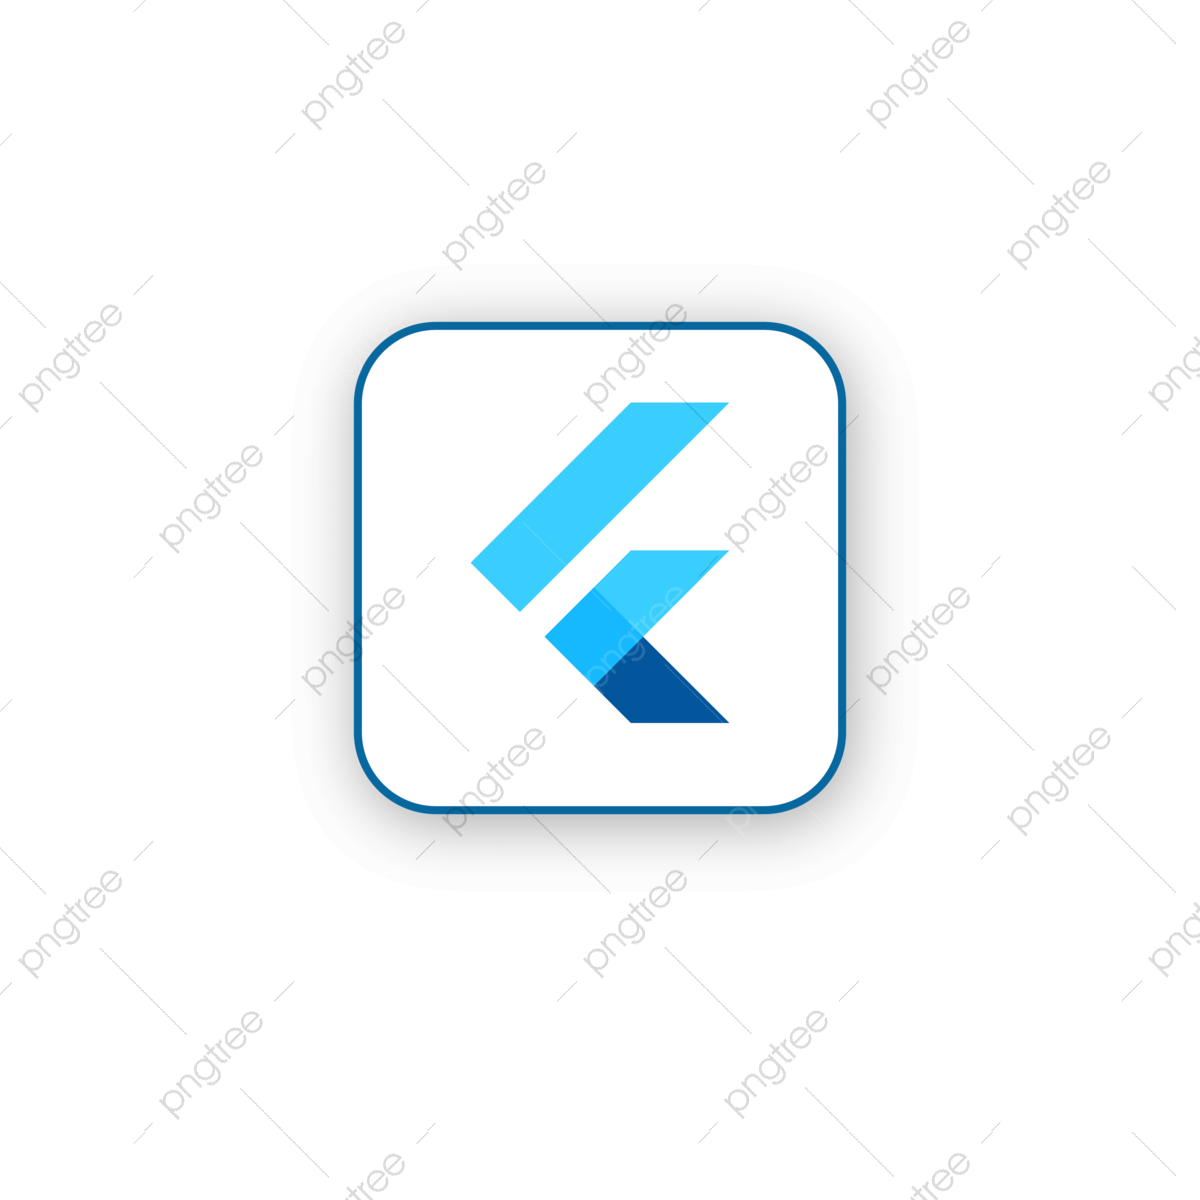
\includegraphics[width=0.5\textwidth]{Hinhve/flutterimg.png}
    \caption{Flutter - Framework phát triển ứng dụng đa nền tảng}
    \label{fig:flutterimg}
\end{figure}

\textbf{Flutter} là một framework phát triển ứng dụng đa nền
tảng (Cross-Platform SDK) dành cho thiết bị di động. Nó cung cấp một hệ sinh thái đầy đủ cho việc phát triển ứng dụng di động hiện đại, bao gồm:
\begin{itemize}
    \item \textbf{Khung giao diện người dùng (UI Framework):} Flutter cung cấp một mô hình giao diện dựa hoàn toàn trên các widget, trong đó mỗi widget đại diện cho một phần tử giao diện từ nhỏ nhất như nút bấm, đoạn văn bản đến toàn bộ màn hình ứng dụng.
    \item \textbf{Danh mục widget phong phú:} Bao gồm cả widget được thiết kế theo chuẩn Material Design (Android) và Cupertino (iOS), giúp ứng dụng hoạt động và hiển thị phù hợp với nền tảng đích.
    \item \textbf{Công cụ phát triển mạnh mẽ:} Hỗ trợ gỡ lỗi, phân tích hiệu năng (performance profiling), tích hợp chặt với các IDE phổ biến (VS Code, Android Studio), và hỗ trợ tính năng nổi bật \textbf{hot reload}.
    \item \textbf{Khả năng đa nền tảng:} Flutter có thể build ứng dụng không chỉ trên thiết bị di động mà còn hỗ trợ máy tính để bàn (desktop), trình duyệt (web), và các nền tảng thử nghiệm như Google Fuchsia.
\end{itemize}

<<<<<<< HEAD
Mục đích của Flutter hướng đến việc dễ dàng triển khai ứng dụng trên bất kỳ nền tảng nào với mã nguồn duy nhất. Nó cho phép phát triển hiệu quả nhờ cấu trúc UI dựa trên các widget khai báo, khả năng tương thích đa nền tảng, máy ảo hỗ trợ \textbf{hot reload}, và đặc biệt là cách tiếp cận \textbf{lập trình phản ứng} (reactive programming). Trong Flutter, giao diện người dùng được xây dựng như một cây widget phản ánh trực tiếp trạng thái của ứng dụng. Khi trạng thái thay đổi, UI sẽ tự động được cập nhật theo cách tối ưu nhất, giúp việc phát triển trở nên nhanh chóng, chính xác và dễ bảo trì. Việc này không chỉ giúp rút ngắn thời gian phát triển mà còn nâng cao trải nghiệm người dùng.
=======
Mục đích của Flutter hướng đến việc dễ dàng triển khai ứng dụng trên bất kỳ nền tảng nào với mã nguồn duy nhất. Nó cho phép phát triển hiệu quả nhờ cấu trúc UI dựa trên widget khai báo, lập trình phản ứng, khả năng tương thích đa nền tảng và máy ảo hỗ trợ hot reload. 
>>>>>>> e99cf771c83e18ae8ecc6bb8d6dc5eff79ee4fb1

\textbf{Lịch sử phát triển:}  
\begin{itemize}
    \item \textbf{2015: } Flutter được phát triển bởi Google và lần đầu tiên được giới thiệu vào năm 2015 với tên gọi "Sky". Khi đó, nó chỉ có một tính năng chính là "Hot Reload" trên thiết bị Android, giúp giảm thời gian phát triển ứng dụng từ 7 phút xuống còn 400ms.
    \item \textbf{5/2017: } Flutter chính thức được phát hành với phiên bản ổn định. Đây là một bước ngoặt quan trọng, khi Flutter trở thành một framework mã nguồn mở, hỗ trợ phát triển ứng dụng cho cả Android và iOS từ một codebase duy nhất. Đồng thời, Flutter cũng bắt đầu được sử dụng trong các ứng dụng thương mại, như Google Pay và Google Earth
    \item \textbf{2018: } Flutter tiếp tục phát triển với sự hỗ trợ mạnh mẽ từ Google. Framework này bắt đầu thu hút sự chú ý của các nhà phát triển trên toàn thế giới nhờ khả năng phát triển nhanh chóng và hiệu suất cao. Các công ty lớn như Alibaba (với ứng dụng Xianyu) và BMW (với ứng dụng MyBMW) bắt đầu áp dụng Flutter cho các dự án của họ
    \begin{figure}[H]
        \centering
        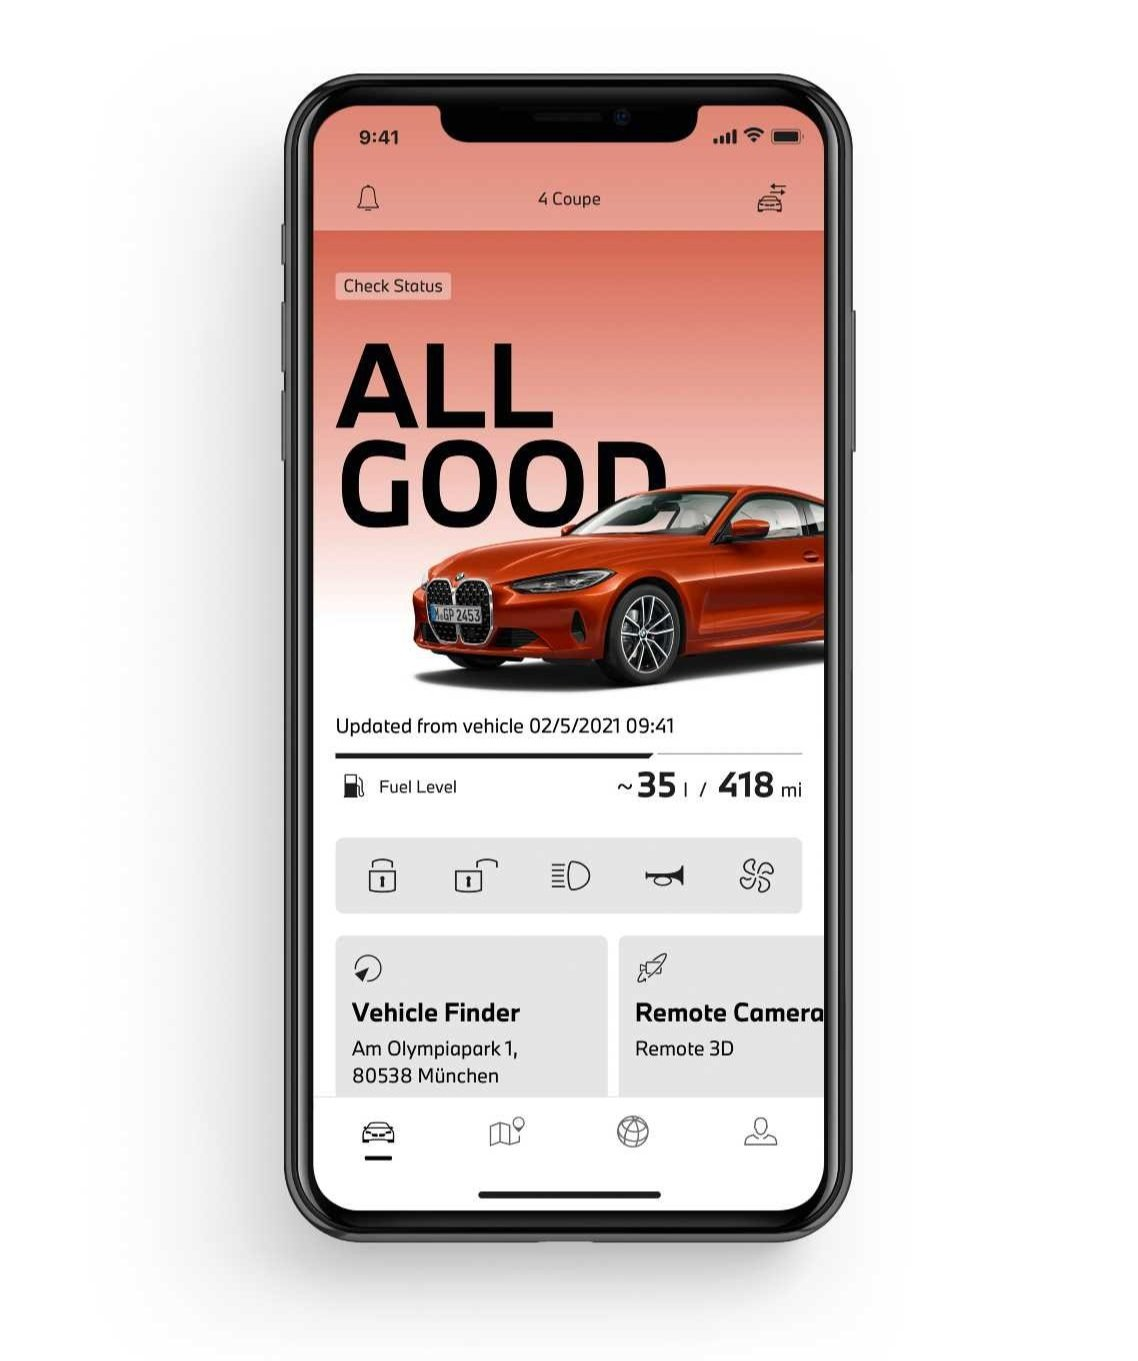
\includegraphics[width=0.6\textwidth]{Hinhve/Chuong5/mybmw.jpg}
        \caption{Giao diện chính app MyBMW - sử dụng Flutter}
        \label{fig:mybmw}
    \end{figure}
    \item \textbf{2020: } Flutter mở rộng hỗ trợ sang các nền tảng khác, bao gồm web, desktop (Windows, macOS, Linux), củng cố vị thế của Flutter như một framework đa nền tảng thực sự.
    \item \textbf{2023: } Theo báo cáo từ Flutter team, hơn một triệu ứng dụng đã được xuất bản sử dụng Flutter, vượt qua tổng số ứng dụng được phát triển trên tất cả các framework đa nền tảng khác cộng lại.
    \item \textbf{Hiện nay (2025): } Flutter tiếp tục được Google hỗ trợ và phát triển, có một hệ sinh thái phong phú với khoảng 37.500 gói thư viện (package) và plugin được chia sẻ trên kho lưu trữ chính thức \texttt{pub.dev}
\end{itemize}

Cộng đồng Flutter vẫn đang phát triển mạnh mẽ cùng với sự đóng góp tích cực từ các lập trình viên trên toàn thế giới ngày càng giúp tăng cường hiệu quả và tính linh hoạt của framework.

\textbf{Đối tượng sử dụng:}

Flutter phù hợp với nhiều nhóm đối tượng, mang lại nhiều lợi ích:
\begin{itemize}
\item \textbf{Lập trình viên mới, chưa có nhiều kinh nghiệm}: Dễ học, dễ cài đặt, không cần kinh nghiệm phát triển di động, với tài liệu chi tiết và cộng đồng hỗ trợ lớn. Theo khảo sát Stack Overflow 2024, 12,4\% lập trình viên đã sử dụng Flutter, và 60,6\% trong số đó muốn tiếp tục sử dụng, cho thấy mức độ phổ biến và sự tin tưởng.

\item \textbf{Lập trình viên Web chuyển sang di động}: Những người quen JavaScript hoặc TypeScript có thể dễ dàng chuyển sang Flutter, tận dụng codebase chung cho Android và iOS, giảm thời gian phát triển. Theo Nomtek Blog, Flutter cho phép tái sử dụng 80-95\% mã nguồn, tiết kiệm chi phí và công sức.

Ví dụ:  Flutter hỗ trợ phát triển web với PWA (Progressive Web Apps), phù hợp cho cửa hàng trực tuyến, trang tin tức, hoặc trang đăng ký, với thiết kế nhất quán và hiệu suất cao

\item \textbf{Doanh nghiệp và startup}: Flutter lý tưởng cho dự án mới để kiểm chứng ý tưởng nhanh chóng nhờ chu kỳ phát triển nhanh và widget sẵn có. Các startup như Nubank, Invoice Ninja, Reflectly đã thành công với Flutter nhờ tính chi phí hiệu quả và tính năng phong phú. Các công ty như Toyota, BMW, eBay, Alibaba, Google (Google Pay, Google Earth, Google Analytics) sử dụng Flutter cho ứng dụng thương hiệu, với lợi ích như giảm thời gian phát triển và giảm kích thước codebase (giảm kích thước 45\%, phát hành nhanh hơn 44\%).

\begin{figure}[H]
    \centering
    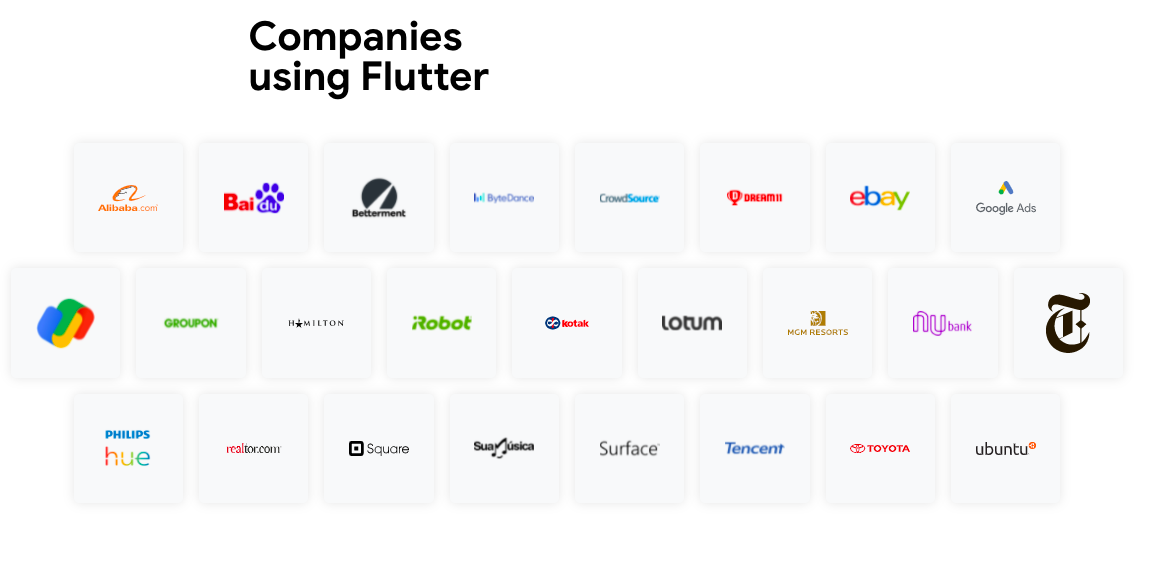
\includegraphics[width=0.75\textwidth]{Hinhve/Chuong5/companyusingflutter.png}
    \caption{Danh sách công ty lớn sử dụng Flutter}
    \label{fig:companyusingflutter}
\end{figure}

\end{itemize}

<<<<<<< HEAD
\textit{Flutter} sử dụng ngôn ngữ lập trình \textbf{Dart} làm nền tảng. \textbf{Dart} cung cấp cú pháp hướng đối tượng gọn gàng cùng hai chế độ biên dịch hiện đại—\emph{ahead-of-time} (AOT) và \emph{just-in-time} (JIT). Các chế độ biên dịch này vừa tối ưu hiệu năng trên thiết bị thật, vừa hỗ trợ \emph{hot reload} để phản hồi tức thời trong giai đoạn phát triển. Bên cạnh đó, cơ chế \emph{Null Safety} của Dart loại trừ lỗi giá trị \texttt{null} ngay khi biên dịch, qua đó nâng độ tin cậy của ứng dụng Flutter.
=======
Flutter sử dụng ngôn ngữ Dart, một ngôn ngữ lập trình hướng đối tượng do Google phát triển. Dart có cú pháp đơn giản, dễ học và hỗ trợ các tính năng hiện đại như:
\begin{itemize}
    \item \textbf{Biên dịch Ahead-of-Time (AOT):} Giúp cải thiện hiệu năng khi chạy ứng dụng trên thiết bị thực.
    \item \textbf{Biên dịch Just-in-Time (JIT):} Hỗ trợ tính năng \textit{Hot Reload}(cho phép cập nhật mã và xem thay đổi tức thì mà không cần triển khai lại ứng dụng) trong quá trình phát triển
    \item \textbf{Null Safety:} Giúp giảm thiểu lỗi liên quan đến giá trị null trong quá trình phát triển ứng dụng.
\end{itemize}
>>>>>>> e99cf771c83e18ae8ecc6bb8d6dc5eff79ee4fb1

Nhờ các đặc điểm trên mà Flutter có thể xây dựng được một ứng dụng chất lượng cao, hiệu năng tốt và giao diện đẹp. Flutter vượt trội so với các nền tảng khác trong việc kiểm soát giao diện, nhất quán giữa các nền tảng.

Ví dụ, một đoạn mã Flutter cơ bản trong Dart có thể trông như sau:
\begin{lstlisting}
import 'package:flutter/material.dart';
void main() {
  runApp(const MyApp());
}
class MyApp extends StatelessWidget {
  const MyApp({Key? key}): super(key: key);
  @override
  Widget build(BuildContext context) {
    return const MaterialApp(
      home: Scaffold(
        body: Center(child: Text('Hello, Flutter!')),
      ),
    );
  }
}
\end{lstlisting}

Đoạn mã này hiển thị dòng chữ \texttt{"Hello, Flutter!"} ở giữa màn hình:
\begin{figure}[H]
    \centering
    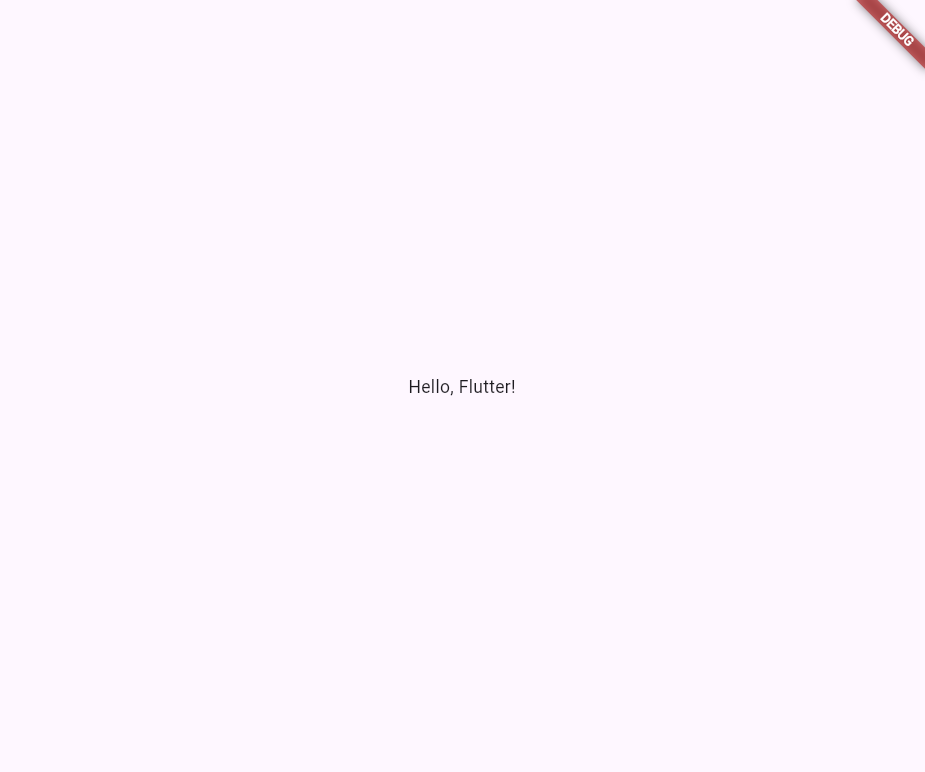
\includegraphics[width=0.9\textwidth]{Hinhve/helloflutter.png}
    \caption{Chương trình minh họa in ra chữ \textit{"Hello, Flutter!"}}
    \label{fig:flutterimg}
\end{figure}

\section{Kiến trúc của Flutter}
<<<<<<< HEAD
\textbf{Flutter} áp dụng mô hình \textbf{kiến trúc phân lớp} nhằm tối ưu hóa khả năng đa nền tảng, hiệu năng và tính mở rộng. Framework này được xây dựng như một hệ thống các thư viện độc lập, trong đó mỗi thư viện chỉ phụ thuộc vào lớp bên dưới. Không có lớp nào có đặc quyền truy cập vào các lớp khác, và mỗi phần của framework được thiết kế để có thể tùy chọn và thay thế. Cấu trúc phân lớp này cho phép các nhà phát triển dễ dàng thêm các tính năng mới hoặc tùy chỉnh các thành phần hiện có để đáp ứng nhu cầu cụ thể của ứng dụng. Mỗi lớp trong kiến trúc Flutter được thiết kế độc lập, giúp giảm thiểu sự phụ thuộc giữa các thành phần, từ đó nâng cao khả năng bảo trì và mở rộng của ứng dụng.

Một khái niệm quan trọng của \textbf{Flutter framework} đó là các thành phần sẽ được nhóm lại theo độ phức tạp và được sắp xếp rõ ràng trong các tầng có độ phức tạp giảm dần. Một \textbf{layer} (tầng, lớp) được tạo thành bằng việc sử dụng các class tiếp theo ngay canh nó. Top của tất cả các layer là các widget đặc biệt cho Android và iOS. Layer tiếp theo là widget gốc của flutter. Tiếp nữa là \textit{Rendering layer}, đây là level thấp nhất trong việc sinh các thành phần của flutter app. Layer tiếp theo là nền tảng gốc hệ điều hành.
=======
\textbf{Flutter} áp dụng mô hình kiến trúc phân lớp nhằm tối ưu hóa khả năng đa nền tảng và hiệu năng, dễ dang mở rộng. Nó tồn tại dưới dạng một loạt các thư viện độc lập mà mỗi thư viện phụ thuộc vào lớp bên dưới. Không có lớp nào có đặc quyền truy cập vào các lớp bên dưới, mỗi phần framework được thiết kế để có thể tùy chọn và thay thế.

Một khái niệm quan trọng của \textbf{Flutter framework} đó là các thành phần sẽ được nhóm lại theo độ phức tạp và được sắp xếp rõ ràng trong các tầng có độ phức tạp giảm dần. Một \textbf{layer} (tầng,lớp) được tạo thành bằng việc sử dụng các class tiếp theo ngay canh nó. Top của tất cả các layer là các widget đặc biệt cho Android và iOS. Layer tiếp theo là widget gốc của flutter. Tiếp nữa là \textit{Rendering layer}, đây là level thấp nhất trong việc sinh các thành phần của flutter app. Layer tiếp theo là nền tảng gốc hệ điều hành.
>>>>>>> e99cf771c83e18ae8ecc6bb8d6dc5eff79ee4fb1

Sơ đồ kiến trúc tổng thể của Flutter được chia thành ba tầng chính: tầng \textbf{Framework} (viết bằng Dart), tầng \textbf{Engine} (viết bằng C/C++) và tầng \textbf{Embedder} (giao tiếp với hệ điều hành)

\begin{figure}[H]
    \centering
    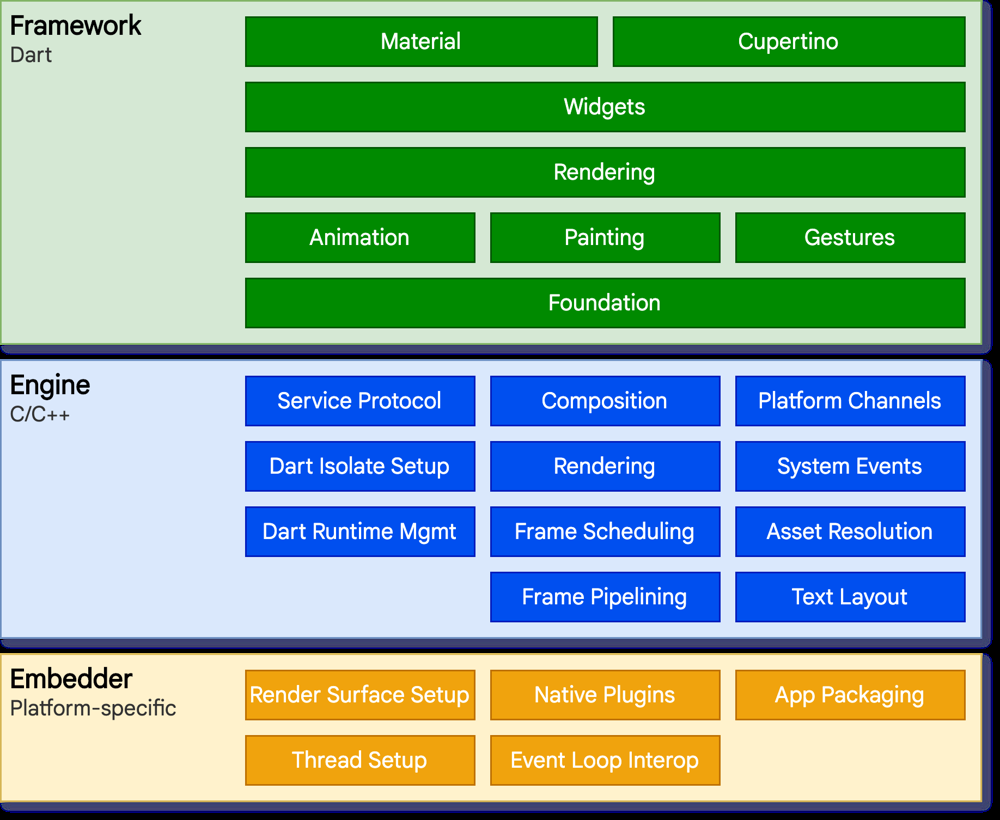
\includegraphics[width=0.9\textwidth]{Hinhve/Chuong5/flutterArchitecture.png}
    \caption{Kiến trúc tổng thể của một ứng dụng Flutter}
    \label{fig:flutterarchitecture}
\end{figure}

\begin{itemize}
\item \textbf{Tầng Framework} cung cấp các thư viện Dart cấp cao để xây dựng giao diện người dùng, bao gồm các thư viện cơ sở như \texttt{foundation}, các dịch vụ nền tảng như \texttt{animation}, \texttt{painting}, \texttt{gestures} và các lớp \texttt{rendering}, \texttt{widgets}, cũng như thư viện giao diện \texttt{Material} và \texttt{Cupertino}.
\item \textbf{Tầng Engine} là lõi của Flutter (hầu hết viết bằng C++), chịu trách nhiệm các tác vụ cấp thấp như raster hóa cảnh thông qua \texttt{Skia}, bố cục văn bản, xử lý I/O và kiến trúc plugin, đồng thời quản lý môi trường thực thi Dart.
\item \textbf{Tầng Embedder} chứa mã gốc riêng theo nền tảng (như Java/Kotlin cho Android, Swift/Objective-C cho iOS) để khởi tạo ứng dụng Flutter, thiết lập bề mặt vẽ đồ họa, vòng lặp sự kiện và tích hợp với các dịch vụ hệ điều hành như nhập liệu và truy cập phần cứng
\end{itemize}
\subsection{Tầng Framework}
 Viết hoàn toàn bằng Dart, tầng Framework nằm phía trên cùng, cung cấp API cao cấp để xây dựng và quản lý giao diện theo mô hình phản ứng.
 \begin{figure}[H]
    \centering
<<<<<<< HEAD
    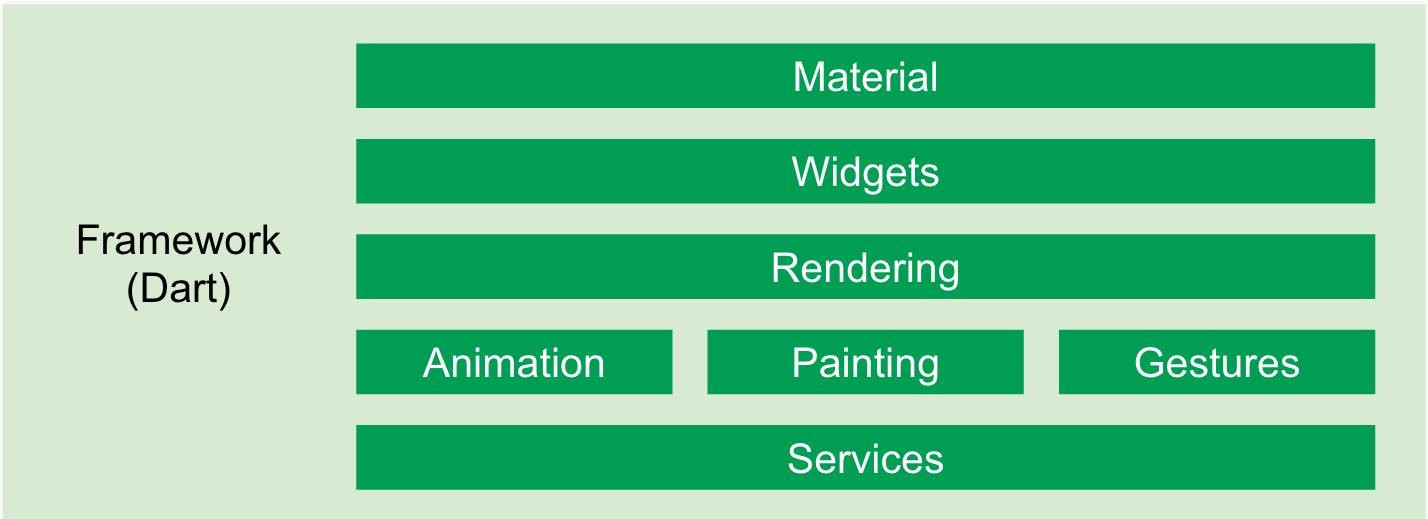
\includegraphics[width=0.9\textwidth]{Hinhve/Chuong5/tang_framework.jpg}
    \caption{Chi tiết về lớp Framework}
    \label{fig:frameworklayer}
=======
    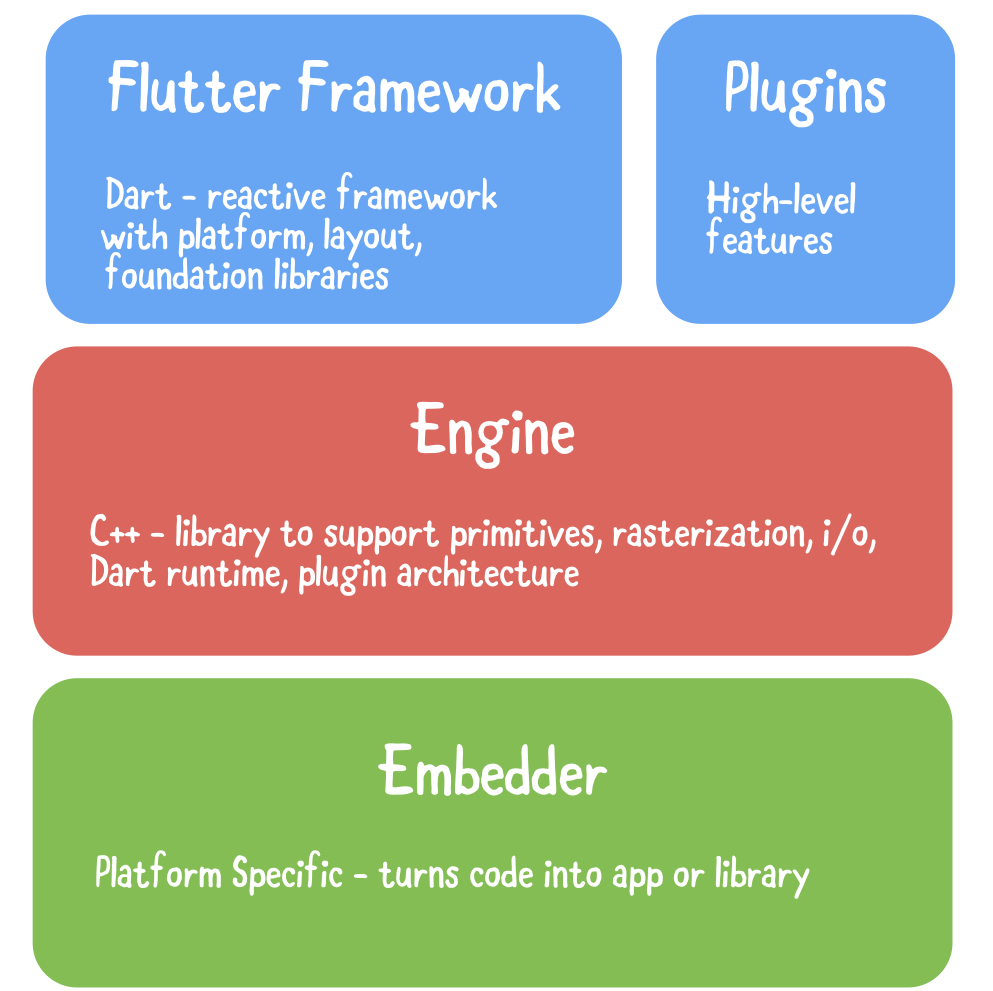
\includegraphics[width=0.9\textwidth]{Hinhve/Chuong5/flutterFramework.png}
    \caption{Chi tiết về lớp Framework}
    \label{fig:flutterframework}
>>>>>>> e99cf771c83e18ae8ecc6bb8d6dc5eff79ee4fb1
\end{figure}
\begin{itemize}
    \item \textbf{Foundation}: Cung cấp các lớp cơ bản và công cụ như error handling, assertions, sử dụng ngôn ngữ thiết kế Material (Android) hoặc Cupertino (iOS).
    \item \textbf{Animation/ Painting/ Gesture}: Thực hiện hoá các chuyển động trong Flutter (Animation), hỗ trợ xây dựng giao diện (Painting), nhận dạng tương tác cử chỉ của người dùng.
    \item \textbf{Rendering Layer}: Quản lý layout và painting, sử dụng \textbf{RenderObject} để xác định cách widgets được hiển thị. Lớp này cung cấp abstraction để xử lý layout, cho phép xây dựng cây các đối tượng renderable, và tự động cập nhật khi có thay đổi
    \item \textbf{Widgets}: Là thành phần cơ bản để xây dựng giao diện trong Flutter, sử dụng kiến trúc cây (widget tree). Nó được xây dựng theo dạng cây với những object là lớp kế thừa của \textbf{RenderObject}. Widgets nhận và lưu trữ trạng thái (state) của UI, và sẽ rebuild nếu state thay đổi.
    \item \textbf{Material/Cupertino}: Được xây dựng từ Widgets library để triển khai ngôn ngữ thiết kế Material (Android) và iOS (Cupertino). Điều này giúp ứng dụng có giao diện native, phù hợp với từng nền tảng
\end{itemize}
\subsection{Tầng Engine (C++):} 
\begin{figure}[H]
    \centering
    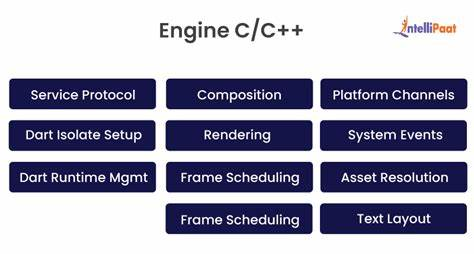
\includegraphics[width=0.9\textwidth]{Hinhve/Chuong5/enginelayer.jpg}
    \caption{Kiến trúc chi tiết lớp Engine}
    \label{fig:enginelayer}
\end{figure}
Tầng Engine là lõi của Flutter, chủ yếu được viết bằng C++ để đảm bảo hiệu suất cao, đặc biệt phù hợp cho các tác vụ cần truy cập trực tiếp vào phần cứng. Nó chịu trách nhiệm xử lý các tác vụ cấp thấp bao gồm:
\begin{itemize}
    \item \textbf{Rasterization:} Quá trình chuyển đổi đồ họa vector thành pixel để hiển thị trên màn hình, sử dụng Impeller trên iOS, Android, desktop (hiện đang thử nghiệm, sau cờ), và Skia trên các nền tảng khác. Skia là thư viện đồ họa 2D nổi tiếng, được Google tích hợp trong Chrome và Android, đảm bảo hiệu suất render tối ưu.
    \item \textbf{Core APIs:} Cung cấp triển khai cho các API cốt lõi:
    \begin{itemize}
        \item \textbf{Graphics:} Không chỉ bao gồm rasterization mà còn xử lý các lệnh vẽ, quản lý texture, và các tác vụ đồ họa khác.
        \item \textbf{Text layout:} Tính toán cách hiển thị văn bản, bao gồm lựa chọn font, kích thước, và định dạng văn bản trên giao diện.
        \item \textbf{File and network I/O:} Hỗ trợ ứng dụng đọc ghi file và thực hiện các yêu cầu mạng, rất cần thiết cho những ứng dụng đòi hỏi kết nối internet.
        \item \textbf{Trợ năng (Accessibility):} Đảm bảo ứng dụng phù hợp cho mọi người dùng, bao gồm cả người khuyết tật, thông qua tích hợp với các công cụ như screen reader, đáp ứng tiêu chuẩn accessibility.
        \item \textbf{Plugin architecture:} Cho phép sử dụng mã native thông qua plugin, mở rộng chức năng ứng dụng như tích hợp camera, GPS, hoặc trình phát video.
        \item \textbf{Dart runtime:} Cung cấp máy ảo Dart để thực thi mã nguồn, hỗ trợ hiệu suất runtime với JIT (Just-In-Time) trong quá trình debug và AOT trong bản release.
        \item \textbf{Compilation toolchain:} Hỗ trợ công cụ biên dịch (AOT compilation), chuyển mã Dart thành mã native nhằm cải thiện tốc độ thực thi, đặc biệt trên các thiết bị di động.
    \end{itemize}
    \item Đóng vai trò trung gian giữa mã nguồn viết bằng Dart và thiết bị phần cứng (hoặc phần mềm bên ngoài ứng dụng).
    \item Thực thi các đoạn mã đã được thông dịch hoặc biên dịch, đồng thời cung cấp các hệ thống runtime như garbage collector và các thư viện cần thiết của ngôn ngữ.
\end{itemize}
<<<<<<< HEAD
\subsection{Tầng \textit{Embedder}}
=======
\subsection{Tầng Embedder} 
>>>>>>> e99cf771c83e18ae8ecc6bb8d6dc5eff79ee4fb1

\begin{figure}[H]
    \centering
    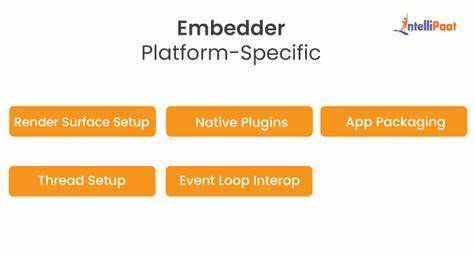
\includegraphics[width=0.9\textwidth]{Hinhve/Chuong5/embedderlayer.jpg}
    \caption{Kiến trúc chi tiết lớp Embedder}
    \label{fig:embedderlayer}
\end{figure}

<<<<<<< HEAD
Tầng \textit{Embedder} tạo cầu nối trực tiếp giữa \textit{Flutter Engine} và hệ điều hành mục tiêu. Cầu nối này được hiện thực khác nhau trên từng nền tảng: ở Android, mã Java hoặc Kotlin nhúng nội dung Flutter vào \textit{Activity}; ở iOS, mã Objective-C hoặc Swift kết xuất giao diện lên \textit{UIViewController}; còn trên Web, mã JavaScript gắn kết engine với \textit{HTML Canvas}.

Nhờ cấu trúc chuyên biệt ấy, tầng \textit{Embedder} đồng thời khởi tạo engine và ngữ cảnh đồ họa, điều phối vòng lặp sự kiện cùng các luồng nền tảng, cũng như trung gian trao đổi dữ liệu giữa Flutter và hệ thống nhập liệu, cảm biến, camera, microphone, GPS cùng mọi dịch vụ bản địa khác.

=======
Là phần gắn kết với hệ điều hành. Mỗi nền tảng lại có embedder riêng. Ví dụ:
\begin{itemize}
    \item Android: dùng Java/Kotlin để hiển thị Flutter trên Activity.
    \item iOS: dùng Objective-C/Swift để render lên UIViewController.
    \item Web: tích hợp với HTML Canvas và JavaScript.
\end{itemize}

Embedder chịu trách nhiệm:
    \begin{itemize}
        \item Khởi tạo engine và môi trường vẽ.
        \item Xử lý vòng lặp sự kiện và luồng.
        \item Giao tiếp với hệ thống nhập liệu, camera, microphone, GPS,...
    \end{itemize}
>>>>>>> e99cf771c83e18ae8ecc6bb8d6dc5eff79ee4fb1

\section{Ứng dụng Flutter đầu tiên}
Với khả năng cross-platform, Flutter cho phép các nhà phát triển tạo ra các ứng dụng hiệu suất cao, sử dụng ngôn ngữ Dart, một ngôn ngữ hiện đại, dễ học và hỗ trợ lập trình hướng đối tượng cũng như lập trình chức năng. Để phát triển ứng dụng Flutter, Android Studio là một trong những công cụ lý tưởng nhất. 

\begin{figure}[H]
    \centering
    
\includegraphics[width=0.6\textwidth]{Hinhve/Chuong5/androidstudio.jpg}
    \caption{Công cụ Android Studio}
    \label{fig:androidstudio}
\end{figure}

Android Studio vốn là môi trường phát triển tích hợp (IDE) chính thức cho ứng dụng Android, nhưng nó cũng được tích hợp chặt chẽ để hỗ trợ Flutter. Nhờ nền tảng mạnh mẽ từ IntelliJ IDEA, Android Studio cung cấp các tính năng vượt trội như:
\begin{itemize}
    \item \textbf{Flutter Inspector: } Giúp kiểm tra và phân tích cấu trúc giao diện người dùng (widget) của ứng dụng.
    \item \textbf{Hot Reload: } Cho phép xem thay đổi mã nguồn ngay lập tức mà không cần khởi động lại ứng dụng, tăng tốc quá trình phát triển.
    \item \textbf{Công cụ debug: } Hỗ trợ tìm và sửa lỗi một cách hiệu quả.
\end{itemize}

Những tính năng này giúp nâng cao năng suất, đặc biệt khi bắt đầu xây dựng ứng dụng Flutter đầu tiên.

\textbf{Cấu trúc của một dự án Flutter:}
Để tạo một dự án Flutter mới trong Android Studio, ta có thể chọn menu \textit{File > New > New Flutter Project} hoặc sử dụng lệnh CLI trong terminal.
\begin{lstlisting}
flutter create <project_name>
\end{lstlisting}
Lệnh trên sẽ sinh ra một cấu trúc dự án cơ bản với một tệp \texttt{pubspec.yaml} và các thư mục cần thiết. Khi build lần đầu, Flutter cũng tạo ra tệp \texttt{pubspec.lock} để khóa phiên bản các gói phụ thuộc, đảm bảo tính tái lập của dự án.
Cấu trúc dự án không chỉ giúp quản lý mã nguồn và tài nguyên một cách khoa học mà còn là nền tảng để ứng dụng hoạt động trơn tru trên các nền tảng khác nhau
Một dự án Flutter điển hình có cấu trúc thư mục như bên dưới:
\begin{figure}[H]
    \centering
    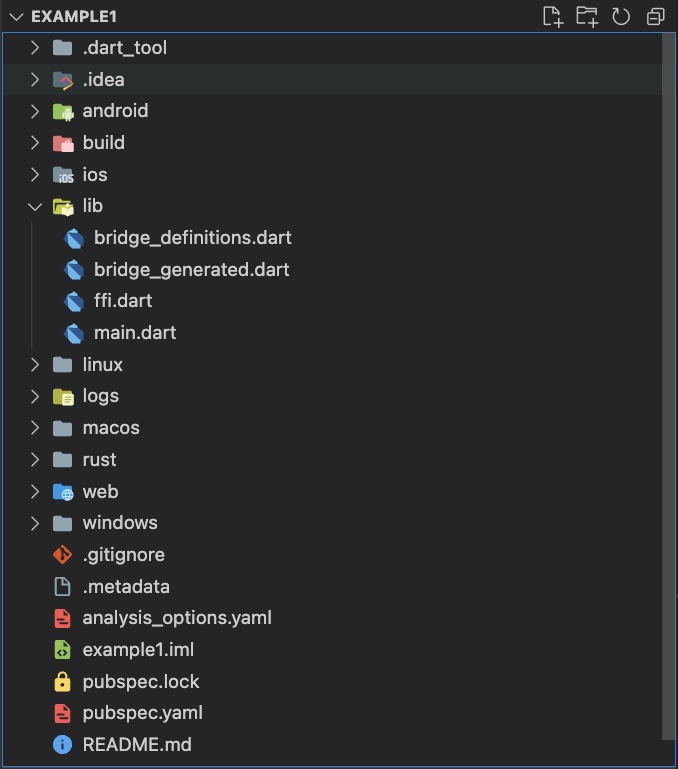
\includegraphics[width=0.8\textwidth]{Hinhve/Chuong5/flutterStructure.png}
    \caption{Cấu trúc của một dự án Flutter}
    \label{fig:flutterstructure}
\end{figure}
Các thư mục và tệp chính bao gồm: 
\begin{itemize}
\item \textbf{{android:}} Thư mục được sinh tự động, chứa mã và cấu hình dành riêng cho nền tảng Android, bao gồm các tệp \textbf{AndroidManifest}, các script \textbf{Gradle}, file cấu hình ứng dụng. Đây là nơi Flutter tích hợp với hệ sinh thái Android.
\item \textbf{{ios:}} Thư mục được sinh tự động, chứa mã và cấu hình dành riêng cho nền tảng iOS, bao gồm dự án \textbf{Xcode}, các tệp \textbf{plist} (Info.plist), và tài nguyên liên quan đến iOS.
\item \textbf{lib:} Thư mục chứa mã Dart của ứng dụng Flutter. Tại đây thường có tệp \texttt{main.dart} làm điểm vào (entry point) của ứng dụng, và có thể chia nhỏ thành các thư mục con để quản lý mã nguồn (widgets, models, services, v.v.), đây là thư mục mà lập trình viên làm việc nhiều nhất.
\item \textbf{{test:}} Folder chứa Dart code, gồm các bài kiểm thử (unit tests, widget tests, integration tests) cho ứng dụng. Mặc định có một số tệp ví dụ và bài kiểm thử mẫu. Thư mục này giúp tổ chức mã kiểm thử riêng biệt với mã ứng dụng.
\item \textbf{{assets (Có thể có):}} Chứa các tài nguyên tĩnh của ứng dụng như hình ảnh, font chữ, hoặc file dữ liệu. Flutter cung cấp hệ thống quản lý tài nguyên qua \texttt{pubspec.yaml}, cho phép truy cập các tài nguyên này trong mã Dart.
\item \textbf{.gitignore:} Git version control file - Đây là file chứa cấu hình cho project git.
\item \textbf{.metadata: } Sinh tự động bởi flutter tools.
\item \textbf{.packages: } Được sinh tự động để theo dõi flutter packages.
\item \textbf{{pubspec.yaml}}: Là tệp cấu hình chính (định dạng YAML) của dự án Flutter. Đóng vai trò như "trái tim", tại đây khai báo metadata của dự án (tên, phiên bản, mô tả), tài nguyên(hình ảnh, font,...) và danh sách các phụ thuộc (packages) cần thiết. Ví dụ, dự án mặc định sẽ có Flutter SDK và gói \texttt{cupertino\_icons} được liệt kê trong \texttt{dependencies}, cùng các phụ thuộc dev.
\end{itemize}

Ngoài ra, tùy vào cấu hình và mục tiêu phát triển, dự án có thể có thêm các thư mục như \textbf{web/} (nếu bật hỗ trợ Web), \textbf{linux/}, \textbf{windows/}, \textbf{macos/} (cho desktop), hoặc thư mục \textbf{build/} chứa các đầu ra biên dịch.

\textbf{Phân tích mã nguồn \texttt{lib/main.dart} của ứng dụng đầu tiên:}

Dưới đây là ví dụ mã nguồn trong file \texttt{lib/main.dart} cho ứng dụng Flutter cơ bản kiểu “Hello World”:

\begin{lstlisting}
import 'package:flutter/material.dart'; 
void main(){
    runApp(const MyApp());
}
class MyApp extends StatelessWidget { 
    const MyApp({super.key});
    @override 
    Widget build(BuildContext context) { 
        return MaterialApp( 
            title: 'Welcome to Flutter', 
            home: Scaffold( 
                appBar: AppBar( 
                    title: Text('Welcome to Flutter'), 
                ), 
                body: const Center( 
                    child: Text('Hello World'), 
                ), 
            ), 
        ); 
    }
}
\end{lstlisting}

Kết quả minh họa của đoạn mã nguồn trên:
\begin{figure}[H]
    \centering
    \includegraphics[width=0.5\textwidth]{Hinhve/Chuong5/demofirstprogram.png}
    \caption{Kết quả của chương trình minh họa}
    \label{fig:flutterstructure}
\end{figure}

Phân tích chi tiết từng thành phần trong đoạn mã trên:

\begin{itemize}
\item \texttt{import 'package:flutter/material.dart';} : Dòng này import thư viện Material Design của Flutter, cho phép sử dụng các widget chuẩn phong cách Material như \texttt{MaterialApp}, \texttt{Scaffold}, \texttt{AppBar}, \texttt{Center}, \texttt{Text}… mà ứng dụng cần. Thư viện này cung cấp các thành phần UI sẵn có để xây dựng giao diện theo phong cách Material Design (của Google).
\item \texttt{void main(){...}} : Điểm khởi đầu của ứng dụng Flutter là hàm \texttt{main()}. Phương thức \texttt{runApp()} được gọi và truyền vào đối tượng của lớp \textbf{\texttt{MyApp}}. Mục đích của phương thức \texttt{runApp()} là để đưa giao diện Widget vào hiển thị trên màn hình.
\item \texttt{class MyApp extends StatelessWidget} : Định nghĩa lớp \texttt{MyApp} kế thừa từ \texttt{StatelessWidget}. Widget được sử dụng để tạo UI(giao diện người dùng). \texttt{StatelessWidget} là loại widget không có trạng thái thay đổi (immutable). nghĩa là nó xây dựng giao diện dựa vào thông tin cố định và sẽ không tự tái tạo khi có sự kiện (nếu cần trạng thái thay đổi ta dùng \texttt{StatefulWidget} thay thế). Do đó, \texttt{MyApp} là thành phần gốc đơn giản của ứng dụng, chịu trách nhiệm trả về widget con trong phương thức \texttt{build()}.
\item \texttt{Widget build (BuildContext context)}: \textbf{\texttt{MyApp}} ghi đè phương thức \texttt{build()}. Mục đích của phương thức \texttt{build()} là tạo một phần UI cho ứng dụng. Đây là nơi định nghĩa cây widget mà \texttt{MyApp} xây dựng. Phương thức trả về một widget, trong trường hợp này là một \texttt{MaterialApp}.
\item \texttt{return MaterialApp(\ldots)}: \texttt{MaterialApp} là widget cấp cao dùng cho ứng dụng theo chuẩn Material Design. Nó bao gồm nhiều cấu hình và widget con cần thiết (như điều hướng, theme, locale), và thường là widget gốc trong các ứng dụng Material. Việc sử dụng \texttt{MaterialApp} giúp dễ dàng tạo giao diện phong cách Material. Trong ví dụ trên, \texttt{MaterialApp} được cấu hình với thuộc tính \texttt{title} (tiêu đề ứng dụng) và \texttt{home} (widget trang chính).  
\begin{itemize} 
\item \texttt{title: 'Welcome to Flutter'}: Dùng để thiết lập tiêu đề ứng dụng. Trên Android, tiêu đề này xuất hiện ở màn hình đa nhiệm (Recent Apps), và trên web nó hiển thị trong tab trình duyệt, còn ở iOS thì giá trị này không được sử dụng để hiển thị vì iOS lấy tên ứng dụng từ file cấu hình \texttt{Info.plist}.
\item \texttt{home: Scaffold(...)}: Thuộc tính \texttt{home} của \texttt{MaterialApp} quy định trang đầu tiên (route mặc định “/”) của ứng dụng.
\end{itemize}

\item \texttt{Scaffold}: Widget \texttt{Scaffold} cung cấp khung bố cục cơ bản cho ứng dụng theo Material Design. Nó tự động thiết lập vùng hiển thị, bao gồm thanh AppBar ở trên, nội dung trong thân, ... Trong ví dụ, \texttt{Scaffold} chứa hai phần chính: 
\begin{itemize} 
\item \texttt{appBar: AppBar(...)}: Thiết lập thanh ứng dụng (App Bar) nằm ở đầu màn hình. Đây là một widget dạng toolbar tiêu chuẩn, có thể chứa tiêu đề, biểu tượng, các nút hành động, v.v. Ở đây, \texttt{AppBar} được tạo với tiêu đề là một widget \texttt{Text} hiển thị chuỗi “Welcome to Flutter”. 
\item \texttt{body: Center(child: Text('Hello World'))}: Đây là phần thân của Scaffold. Ở ví dụ này, \texttt{body} là một widget \texttt{Center}, nhằm căn giữa nội dung con của nó. Bên trong \texttt{Center}, có một widget \texttt{Text} để hiển thị văn bản “Hello World”.
\end{itemize}

\item Các thành phần con khác: 
\begin{itemize} 
\item \texttt{const MyApp({super.key};)} : Định nghĩa constructor hằng (const constructor) cho lớp \texttt{MyApp}. Sử dụng \texttt{const} giúp Flutter tối ưu hóa xây dựng widget (có thể tạo các instance hằng) khi tham số không đổi. Tham số \texttt{key} được truyền lên lớp cha để quản lý trong cây widget. \item \texttt{@override}: Ghi chú override phương thức \texttt{build}. Từ khoá này giúp kiểm tra rằng lớp con đang ghi đè đúng phương thức của lớp cha. 
\item \texttt{ThemeData(primarySwatch: Colors.blue)}: Thiết lập chủ đề (theme) cho ứng dụng, ví dụ màu chính của Material. (Ở ví dụ trên, ta không đặt theme riêng, nên màu mặc định sẽ là màu trắng)
\end{itemize}
\end{itemize}

\section{Flutter widgets}
\subsection{Giới thiệu khái niệm Widget trong Flutter}
Trong Flutter, giao diện người dùng được xây dựng hoàn toàn từ các \textit{widget}. Widget là thành phần cơ bản nhất tạo nên toàn bộ giao diện người dùng của ứng dụng Flutter. Mỗi widget là một lớp định nghĩa một phần cấu hình giao diện. Một widget biểu diễn cách mà màn hình nên hiển thị trong một trạng thái nhất định. Hầu hết mọi thứ nhìn thấy như hình ảnh, biểu tượng, văn bản đều là widget; thậm chí các thành phần dùng để bố cục như \texttt{Row}, \texttt{Column}, \texttt{Container} cũng là widget.

Bằng cách kết hợp (compose) các widget đơn giản, Flutter cho phép tạo ra các giao diện phức tạp một cách linh hoạt. Ứng dụng là một top-level widget bao gồm một hoặc nhiều widget con. Trong bản thân mỗi widget lại có thể chứa một hoặc nhiều widget con khác.

Các widget do người dùng định nghĩa sẽ là lớp con của \texttt{StatelessWidget} hoặc \texttt{StatefulWidget} tùy vào việc widget đó có cần lưu trữ trạng thái hay không

\subsection{Phân loại widgets trong Flutter}
Flutter cung cấp nhiều loại widget khác nhau tùy mục đích sử dụng. Widgets có thể là:
\begin{itemize}
\item \textbf{Một phần tử cấu trúc:} Đây là những widgets được sử dụng để xây dựng các thành phần giao diện cơ bản (nút, menu, appbar,...). Các widget này giúp tạo ra các yếu tố tương tác trong giao diện người dùng.
\item \textbf{Một phần tử kiểu dáng (styling elements)}: 
    Flutter hỗ trợ các widget và thuộc tính giúp kiểm soát kiểu dáng toàn cục hoặc cục bộ, bao gồm:
    \begin{itemize}
        \item \texttt{Theme} và \texttt{ThemeData}: Dùng để định nghĩa giao diện tổng thể của toàn bộ ứng dụng như màu sắc, font, kích thước chữ, v.v.
        \item \texttt{DefaultTextStyle}: Thiết lập kiểu chữ mặc định cho tất cả các widget con.
        \item \texttt{TextStyle}: Dùng để định nghĩa cụ thể font chữ, kích thước, màu sắc cho các thành phần văn bản.
        \item \texttt{Padding}, \texttt{Margin}, \texttt{BoxDecoration}: Dùng để thiết lập khoảng cách và hiệu ứng đồ họa.
    \end{itemize}
    Việc sử dụng đúng các widget kiểu dáng giúp đảm bảo tính thống nhất, dễ bảo trì và tái sử dụng trong toàn bộ ứng dụng.
\item \textbf{Một đặc trưng của Layout:} Ví dụ như \texttt{Padding}, \texttt{Align}, \texttt{Center}, \texttt{Margin}, \texttt{Theme}. Các widget này không trực tiếp hiển thị dữ liệu nhưng có tác dụng điều chỉnh vị trí, khoảng cách, căn chỉnh hoặc kiểu dáng của các widget con. 
\end{itemize}

\textit{Ví dụ:}
Đoạn mã dưới đây minh họa việc tạo một widget tùy chỉnh có áp dụng kiểu dáng bằng cách sử dụng \texttt{Padding} và \texttt{TextStyle}:

\begin{lstlisting}
class PaddedText extends StatelessWidget {
  final String _data;

  PaddedText(this._data, {Key? key}) : super(key: key);

  @override
  Widget build(BuildContext context) {
    return Padding(
      padding: const EdgeInsets.all(12.0),
      child: Text(
        _data,
        style: const TextStyle(
          fontSize: 18,
          color: Colors.blue,
          fontWeight: FontWeight.bold,
        ),
      ),
    );
  }
}
\end{lstlisting}

Ở chương trình ví dụ trên:
\begin{itemize}
    \item \texttt{Padding}: Là phần tử layout, dùng để tạo khoảng cách xung quanh widget con của nó, trong ví dụ này, Padding tạo ra khoảng cách 12.0 pixel ở tất cả các hướng xung quanh widget Text
    \item \texttt{Text}: Là phần tử cấu trúc, dùng để hiển thị văn bản là biến \texttt{\_data}
    \item \texttt{TextStyle}: Là một phần tử kiểu dáng, dùng để áp dụng kiểu dáng cho văn bản: màu xanh dương, in đậm, cỡ chữ 18.
\end{itemize}
\textbf{Sơ đồ cấu trúc Widget:}

Cấu trúc widget của ứng dụng Hello World thể hiện mối quan hệ cha con chặt chẽ. Mỗi widget cha cung cấp ngữ cảnh hoặc thuộc tính cho widget con của nó. \textbf{MaterialApp} cung cấp \texttt{home} cho \textbf{MyHomePage}, \textbf{Scaffold} cung cấp \texttt{appBar} và \texttt{body} cho \textbf{AppBar} và \textbf{Center}, \textbf{Center} cung cấp \texttt{child} cho \textbf{Text}.

Flutter render UI bằng cách duyệt qua cây widget từ gốc (\textbf{MyApp}) đến lá (\textbf{Text}), tạo ra một cây render (render tree) dựa trên các widget này.
\begin{figure}[H]
    \centering
    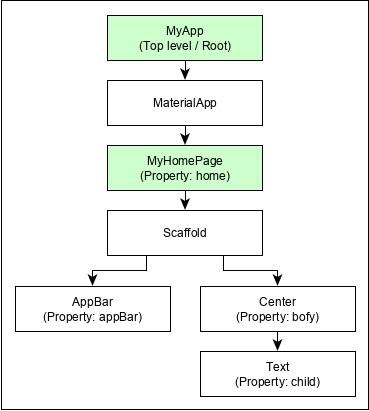
\includegraphics[width=0.5\textwidth]{Hinhve/Chuong5/flutterwidgetsstructure.png}
    \caption{Cấu trúc widget của ứng dụng \textit{Hello World}}
    \label{fig:flutterwidgetsstructure}
\end{figure}
\subsection{Một số widgets phổ biến trong Flutter}
Đây là các thành phần cơ bản giúp tạo cấu trúc ứng dụng như nút, biểu tượng, trường nhập liệu, menu...
\begin{itemize}
\item \textbf{Button: } Buttons cung cấp cho người dùng khả năng thực hiện các hành động, đưa ra lựa chọn, gửi biểu mẫu, lưu dữ liệu, mở trang mới,... bằng cách click vào nó. Nút được phân loại thành nhiều loại: \textbf{Elevated Button}, \textbf{Floating Action Button}, \textbf{Outlined Button}, \textbf{Icon Button}, \textbf{Text Button},...

\textit{Ví dụ:}
\begin{lstlisting}
ElevatedButton(
    onPressed: () {
        print('Clicked'); 
    },
    style: ElevatedButton.styleFrom(
        backgroundColor: Colors.blue, 
    ),
    child: Text('Login'),
),
\end{lstlisting}

Hình ảnh minh họa:
\begin{figure}[H]
    \centering
    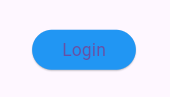
\includegraphics[width=0.9\textwidth]{Hinhve/Chuong5/buttonWidget.png}
    \caption{Elevated Button trong Flutter}
    \label{fig:buttonwidget}
\end{figure}
<<<<<<< HEAD

Trong mỗi Widget lại có các properties riêng biệt, giúp cho bản thân nó trở nên sinh động hơn khi hiển thị ra giao diện. Dưới đây là ví dụ về một số thuộc tính điển hình của widget \textbf{\texttt{ElevatedButton}}:

\begin{table}[H]
\centering
\begin{tabular}{|>{\centering\arraybackslash}p{4cm}|>{\centering\arraybackslash}p{9cm}|}
\hline
\textbf{Thuộc tính} & \textbf{Mô tả thuộc tính} \\ \hline
\texttt{autofocus} & Nhận vào giá trị boolean xác định nút có được focus mặc định khi hiển thị hay không \\ \hline
\texttt{clipBehaviour} & Xác định nội dung của nút có bị cắt (clip) nếu vượt quá kích thước không \\ \hline
\texttt{focusNode} & Đại diện cho node focus của widget \\ \hline
\texttt{ButtonStyle} & Xác định kiểu hiển thị (style) của nút \\ \hline
\texttt{onLongPress} & Hành động sẽ thực hiện khi người dùng nhấn giữ nút \\ \hline
\texttt{enabled} & Nhận vào giá trị boolean xác định nút có hoạt động hay không \\ \hline
\texttt{hashcode} & Xác định mã băm (hashcode) của nút \\ \hline
\texttt{Key} & Điều khiển cách một widget thay thế widget khác trong cây widget \\ \hline
\texttt{onFocusChanged} & Hàm sẽ được gọi khi focus của nút thay đổi \\ \hline
\texttt{onHover} & Hành động được thực hiện khi người dùng di chuột qua nút \\ \hline
\end{tabular}
\caption{Các thuộc tính của ElevatedButton trong Flutter}
\label{tab:elevated_button_properties}
\end{table}

=======
>>>>>>> e99cf771c83e18ae8ecc6bb8d6dc5eff79ee4fb1
\item \textbf{TextField:} Cho phép người dùng nhập văn bản. Được sử dụng rộng rãi trong các biểu mẫu đăng nhập, đăng ký, tìm kiếm, bình luận,...

\textit{Ví dụ:}
\begin{myverbatim}
TextField(
  decoration: InputDecoration(
    border: OutlineInputBorder(),
    labelText: 'Họ tên',
    hintText: 'Nhập họ và tên',
    prefixIcon: Icon(Icons.person),
  ),
),
\end{myverbatim}

Trong ví dụ trên, màn hình hiển thị một trường nhập liệu có biểu tượng \texttt{Icons.email}, nhãn \textit{“Email”}, khung viền và gợi ý nhập liệu.

Hình ảnh minh họa:
\begin{figure}[H]
    \centering
    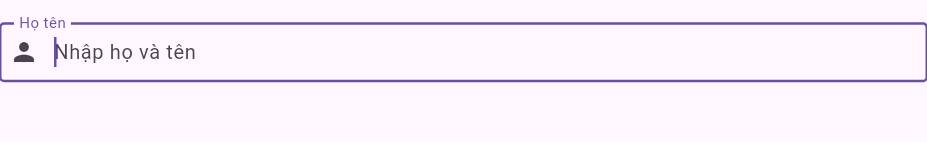
\includegraphics[width=0.8\textwidth]{Hinhve/Chuong5/textfieldWidget.png}
    \caption{Textfield trong Flutter}
    \label{fig:textfieldwidget}
\end{figure}

\item \textbf{Checkbox:} Widget này cho phép người dùng chọn hoặc bỏ chọn một tùy chọn. Thường được sử dụng trong các biểu mẫu hoặc danh sách tùy chọn.

\textit{Ví dụ:}
\begin{lstlisting}
Checkbox(
  value: isChecked,
  onChanged: (bool? newValue) {
    setState(() {
      isChecked = newValue!;
    });
  },
)
\end{lstlisting}


Trong ví dụ trên, màn hình hiển thị một ô checkbox, \texttt{value} cho biết trạng thái hiện tại của checkbox (đã được chọn hay chưa), khi thay đổi trạng thái thì hàm \texttt{onChanged} sẽ được gọi.

\begin{figure}[H]
    \centering
    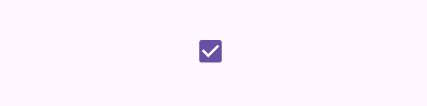
\includegraphics[width=0.9\textwidth]{Hinhve/Chuong5/checkboxWidget.png}
    \caption{Checkbox trong Flutter}
    \label{fig:checkboxwidget}
\end{figure}

\item \textbf{Text: }
Widget Text là một thành phần cơ bản trong Flutter, được sử dụng để hiển thị văn bản trên giao diện người dùng

\textit{Ví dụ:}

\begin{lstlisting}
Text(
    'Hello world!',
     style: TextStyle(
        color: Colors.black,
        fontSize: 40,
        backgroundColor: Colors.white,
        fontWeight: FontWeight.bold,
    ),
)
\end{lstlisting}

Trong ví dụ trên, tham số đầu tiên là một chuỗi văn bản, đây là nội dung văn bản sẽ được hiển thị trên màn hình, tham số \texttt{style} để định dạng kiểu của văn bản. Văn bản hiển thị sẽ có kích cỡ chữ 40 (logical pixels), màu đen, màu nền văn bản màu trắng, độ đậm bold.
\begin{figure}[H]
    \centering
    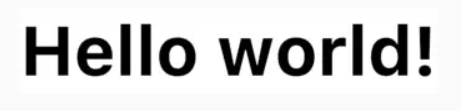
\includegraphics[width=0.5\textwidth]{Hinhve/Chuong5/vd1_text.png}
    \caption{Minh họa về widget Text}
    \label{fig:vd1_text}
\end{figure}

\item \textbf{Row}: Dùng để sắp xếp các widget con theo chiều ngang, thường được sử dụng để hiển thị các thành phần nằm cạnh nhau. Row có tham số bắt buộc là \texttt{children} để chứa các widget con, thứ tự đặt vào trong \texttt{children} sẽ ảnh hưởng tới thứ tự các widget đó xuất hiện trên màn hình.

\textit{Ví dụ:}

\begin{lstlisting}
Row(
  mainAxisAlignment: MainAxisAlignment.center,
  children: const [
    Text('Hello'),
    Text('Flutter!'),
    Text('!!'),
  ],
)
\end{lstlisting}

Kết quả minh họa của chương trình trên:
\begin{figure}[H]
    \centering
    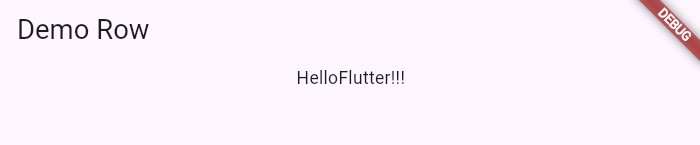
\includegraphics[width=0.9\textwidth]{Hinhve/Chuong5/rowWidget.png}
    \caption{Minh họa về widget Row}
    \label{fig:rowwidget}
\end{figure}

Bên cạnh đó, tham số \texttt{mainAxisAlignment} sẽ ảnh hưởng đến vị trí hiển thị của các widget trong \texttt{children}:
\begin{itemize}
\item \texttt{MainAxisAligment.center}: Các items sẽ nằm ở giữa hàng
\begin{figure}[H]
    \centering
    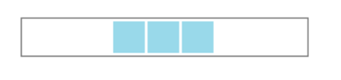
\includegraphics[width=0.9\textwidth]{Hinhve/Chuong5/mainAxAlcenter.png}
    \caption{Thuộc tính \textit{mainAxisAlignment} có giá trị \textit{center}}
    \label{fig:rowwidget(center)}
\end{figure}
\item \texttt{MainAxisAligment.start}: Các items sẽ nằm ở vị trí bắt đầu của hàng đó.
\begin{figure}[H]
    \centering
    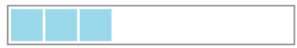
\includegraphics[width=0.9\textwidth]{Hinhve/Chuong5/mainAxAlstart.png}
    \caption{Thuộc tính \textit{mainAxisAlignment} có giá trị \textit{start}}
    \label{fig:rowwidget(start)}
\end{figure}

Tương tự, nếu \texttt{mainAxisAlignment} là \texttt{end} thì các phần tử sẽ được sắp xếp ở cuối hàng đó.
\item \texttt{MainAxisAligment.spaceBetween}: Các items cách đều nhau, phần tử đầu và cuối sẽ ở 2 lề của Row đó.
\begin{figure}[H]
    \centering
    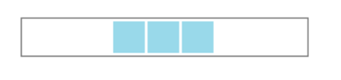
\includegraphics[width=0.9\textwidth]{Hinhve/Chuong5/mainAxAlspace.png}
    \caption{Thuộc tính \textit{mainAxisAlignment} có giá trị \textit{spaceBetween}}
    \label{fig:rowwidget(end)}
\end{figure}
\end{itemize}

\item \textbf{Column:} Column là một widget trong thư viện widgets của Flutter, thuộc nhóm layout widgets, giúp sắp xếp các widget con theo một ngăn xếp dọc. Trục chính (main axis) của Column là trục dọc (vertical), nghĩa là các widget con được xếp từ trên xuống dưới. Trục phụ (cross axis) là trục ngang (horizontal), dùng để căn chỉnh các widget con theo chiều ngang.

\textit{Ví dụ:}
\begin{lstlisting}
Column(
  mainAxisAlignment: MainAxisAlignment.center,
  children: <Widget>[
    Text("Element 1"),
    Text("Element 2"),
    Text("Element 3"),
  ],
),
\end{lstlisting}

\textbf{{Column}} gồm 3 widget \textbf{Text} bên trong nó và \texttt{mainAxisAlignment} được đặt thành \texttt{center}, có nghĩa là các widget con được căn giữa theo chiều dọc.
\begin{figure}[H]
    \centering
    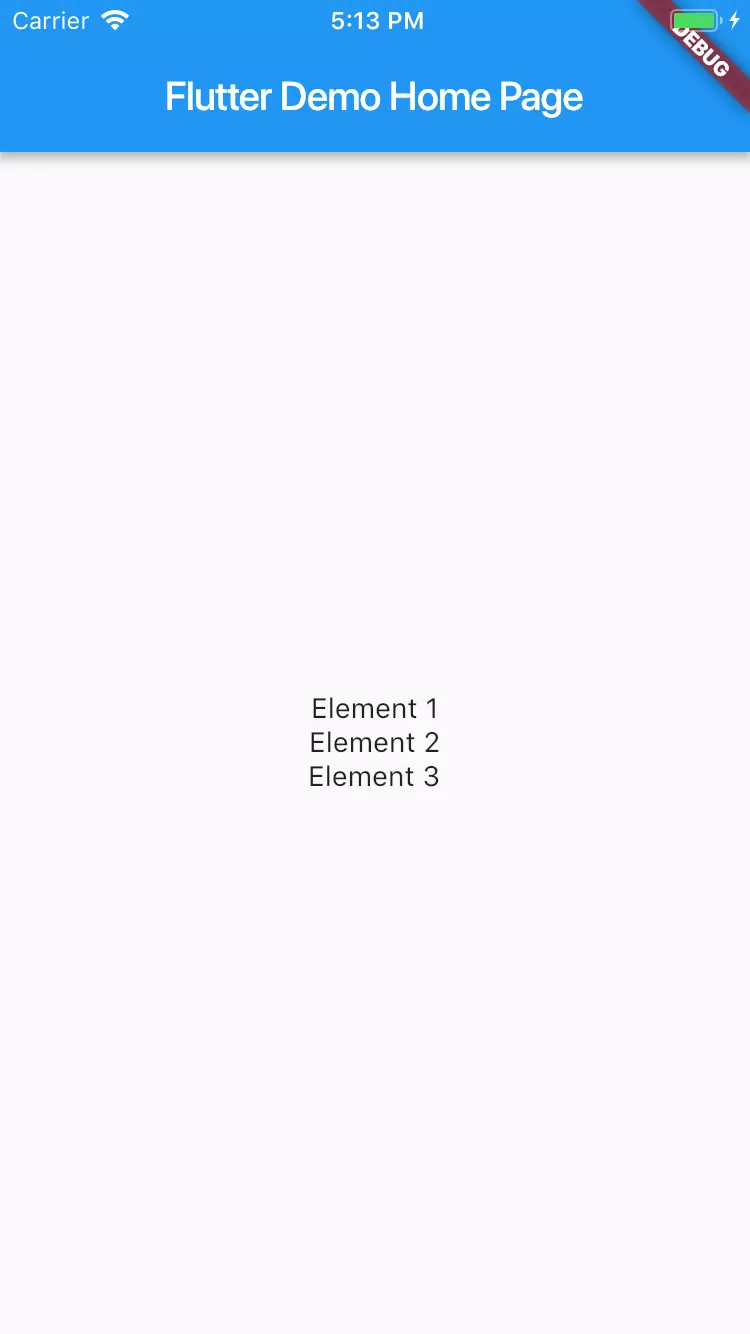
\includegraphics[width=0.5\textwidth]{Hinhve/Chuong5/columnWidget.png}
    \caption{Minh họa về widget Column}
    \label{fig:columnwidget}
\end{figure}

\item \textbf{ListView:} Widget này cho phép hiển thị danh sách các widget con có thể cuộn được theo chiều dọc hoặc ngang, thường được sử dụng để hiển thị danh sách dài các mục.

\begin{figure}[H]
    \centering
    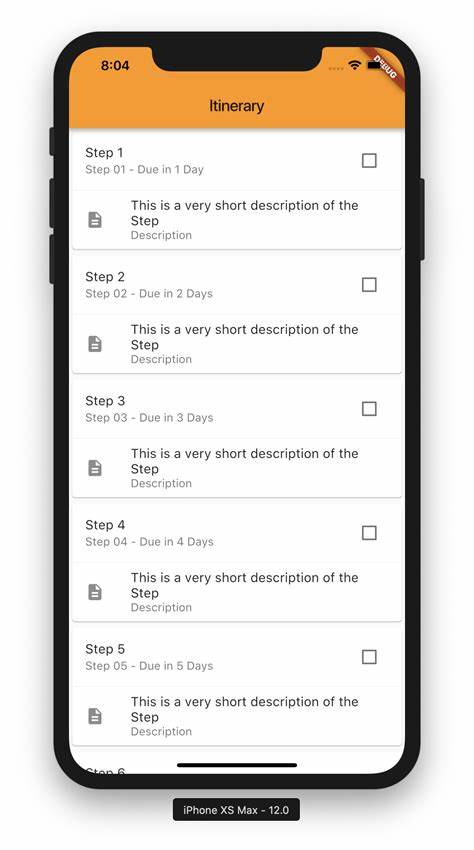
\includegraphics[width=0.5\textwidth]{Hinhve/Chuong5/listview.jpg}
    \caption{Minh họa về widget ListView}
    \label{fig:listviewwidget}
\end{figure}

\textit{Ví dụ:}

\begin{lstlisting}
ListView(
  children: <Widget>[
    ListTile(title: Text('Element 1')),
    ListTile(title: Text('Element 2')),
    ListTile(title: Text('Element 3')),
  ],
)
\end{lstlisting}


Trong ví dụ trên, \texttt{ListView} là widget danh sách cuộn, gồm 3 widget con là \texttt{ListTile} hiển thị nội dung văn bản.

\item \textbf{Stack:} Cho phép chồng các widget con lên nhau, thường được sử dụng để tạo giao diện phức tạp với các thành phần chồng lấp.

\begin{figure}[H]
    \centering
    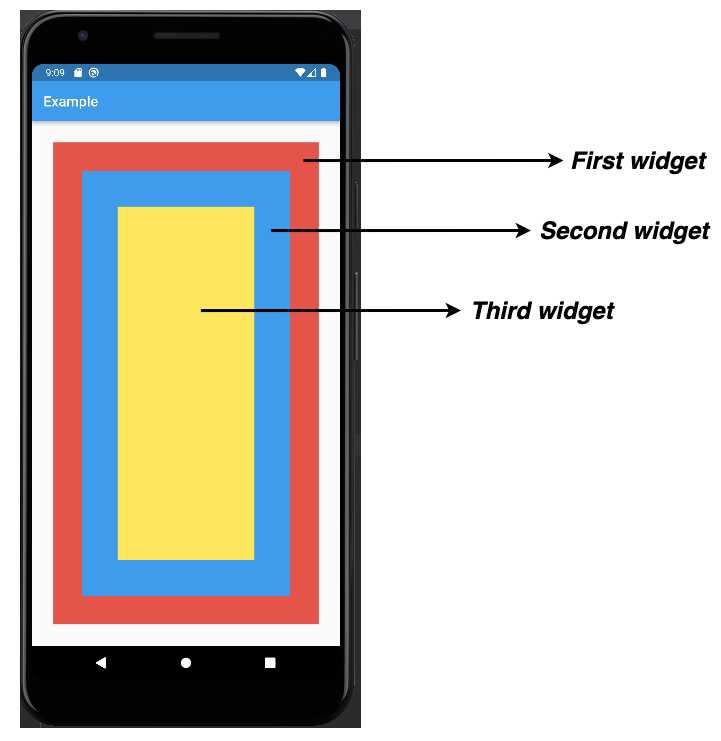
\includegraphics[width=0.6\textwidth]{Hinhve/Chuong5/stackWidget.png}
    \caption{Minh họa về widget Stack}
    \label{fig:stackwidget}
\end{figure}

\textit{Ví dụ:}
\begin{lstlisting}
Stack(
  children: <Widget>[
    Container(width:90, height:90, color:Colors.red),
    Positioned(
      top: 10,
      left: 10,
      child: Container(
        width: 80, 
        height: 80, 
        color: Colors.green
      ),
    ),
  ],
)
\end{lstlisting}

Kết quả của đoạn mã là một giao diện hiển thị một hình vuông màu đỏ 90x90 pixel với một hình vuông màu xanh lá 80x80 pixel được định vị cách mép trái và mép trên 10 pixel, trong đó hình vuông màu xanh chồng lấp lên trên hình vuông đỏ.

\item \textbf{Scaffold:} Cung cấp cấu trúc cơ bản cho một màn hình ứng dụng, bao gồm AppBar, Body, Drawer, BottomNavigationBar,...

\begin{figure}[H]
    \centering
    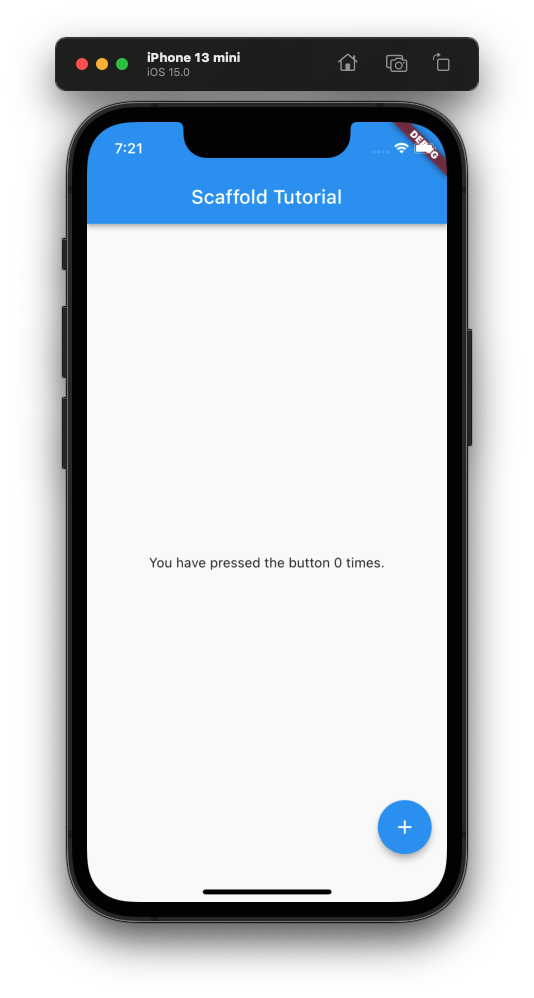
\includegraphics[width=0.6\textwidth]{Hinhve/Chuong5/scaffold.png}
    \caption{Minh họa về widget Scaffold}
    \label{fig:scaffold}
\end{figure}

\textit{Ví dụ:}
\begin{lstlisting}
Scaffold(
  appBar: AppBar(title: Text('Title')),
  body: Center(child: Text('Main Content')),
  floatingActionButton: FloatingActionButton(
    onPressed: () {},
    child: Icon(Icons.add),
  ),
)    
\end{lstlisting}

Trong ví dụ trên, Scaffold gồm 3 tham số chính là \texttt{appBar}: thanh tiêu đề ở đầu màn hình, \texttt{body}: nội dung chính của màn hình, và nút nổi lên trên màn hình (\texttt{floatingActionButton})
\end{itemize}

\subsection{Cách tiếp cận khai báo trong Flutter}

\textbf{Lập trình mệnh lệnh (Imperative):} Trong phong cách này, lập trình viên mô tả từng bước cụ thể để đạt được kết quả mong muốn. Ví dụ, để cập nhật giao diện, ta cần xác định và thao tác trực tiếp với các thành phần UI, như tìm kiếm widget bằng ID và thay đổi thuộc tính của nó.

\textbf{Lập trình khai báo (Declarative):} Ngược lại, lập trình khai báo tập trung vào việc mô tả \textit{giao diện nên trông như thế nào} dựa trên trạng thái hiện tại. Khi trạng thái thay đổi, hệ thống tự động cập nhật giao diện để phản ánh sự thay đổi đó, mà không cần chỉ định các bước cụ thể để thực hiện.

Flutter áp dụng mô hình UI khai báo (declarative), có nghĩa là:

\textit{
"Đây là trạng thái hiện tại của ứng dụng, hãy trả về thứ gì đó trên màn hình cho phù hợp tương ứng trạng thái đó".
}

Giao diện người dùng (UI) trong Flutter được mô hình hóa như một hàm của trạng thái:
\begin{figure}[H]
    \centering
    
\includegraphics[width=0.5\textwidth]{Hinhve/Chuong5/flutterState.jpg}
    \caption{Mô hình hóa hàm trạng thái}
    \label{fig:flutterstate}
\end{figure}
Trong đó \textbf{UI} là giao diện người dùng được hiển thị trên màn hình, có thể quan sát được, còn \textbf{state} là trạng thái hiện tại của ứng dụng, ví dụ như giá trị của một biến hoặc dữ liệu người dùng nhập.

Flutter áp dụng \textbf{mô hình khai báo}, nơi giao diện được xây dựng dựa trên trạng thái ứng dụng. Điều này giúp đơn giản hóa việc quản lý giao diện và giảm thiểu lỗi, vì không cần xử lý các bước cập nhật UI một cách thủ công .

Cách tiếp cận khai báo giúp đơn giản hóa việc quản lý giao diện người dùng và giảm thiểu lỗi, vì Flutter tự động cập nhật UI khi trạng thái thay đổi. Thay vì điều khiển từng bước như trong cách tiếp cận mệnh lệnh, chỉ cần khai báo trạng thái mong muốn, và Flutter sẽ xử lý phần còn lại. Theo tài liệu chính thức của Flutter, cách tiếp cận này giúp tăng hiệu quả phát triển và đảm bảo tính nhất quán của giao diện. Bên cạnh đó, nó đảm bảo chỉ có một đường dẫn mã cho bất kỳ trạng thái nào của giao diện người dùng, điều này giúp dễ dàng kiểm soát và gỡ lỗi, dễ dàng bảo trì và mở rộng giao diện khi ứng dụng có trạng thái phức tạp hơn.

Flutter sử dụng phương thức \texttt{build()} của widget để dựng giao diện người dùng. Nói cách khác, giao diện được coi là một hàm của trạng thái hiện tại, tương ứng với công thức UI = f(state) – tức là, mỗi khi trạng thái (state) thay đổi, Flutter tự động gọi lại build() để xây dựng lại cây widget phù hợp với trạng thái mới. 

\texttt{build()} là phương thức trừu tượng trong lớp Widget (thường được override trong StatelessWidget hoặc trong lớp State của StatefulWidget), nhận một đối tượng BuildContext và trả về một Widget (hoặc cây widget con) mô tả cấu trúc giao diện. Flutter gọi \texttt{build()} trong các tình huống sau:
\begin{itemize}
\item Khi widget được chèn vào cây widget lần đầu tiên.
\item Sau khi gọi \texttt{setState()}, báo hiệu rằng trạng thái đã thay đổi.
\item Khi các widget kế thừa mà widget phụ thuộc vào thay đổi.
\item Sau khi gọi \texttt{didUpdateWidget()} hoặc \texttt{deactivate()} và widget được chèn lại vào cây.
\end{itemize}
\textbf{Nguyên tắc hoạt động:} Mỗi lần \texttt{build()} được gọi, nó phải trả về một cấu trúc widget mới phản ánh trạng thái hiện tại. Flutter sau đó so sánh cây widget mới với cây cũ và cập nhật giao diện một cách hiệu quả 

Ví dụ minh họa phương thức \texttt{build()} và cây widget:

Xét ví dụ dưới đây về một widget đơn giản:
\begin{lstlisting}
class MyHomePage extends StatelessWidget {
    MyHomePage({Key key, this.title}) : super(key: key);
    final String title;
    @override
    Widget build(BuildContext context) {
        return Scaffold(
            appBar: AppBar(title: Text(this.title)),
            body: Center(child: Text('Hello World')),
        );
    }
}    
\end{lstlisting}

Đây là một ví dụ điển hình thể hiện rõ cách Flutter sử dụng phương pháp xây dựng giao diện thông qua \texttt{build()} – định nghĩa giao diện dựa trên dữ liệu trạng thái (ở đây là biến \texttt{title}) và cấu trúc cây widget. Cây widget được xây dựng như sau:
\begin{figure}[H]
    \centering
    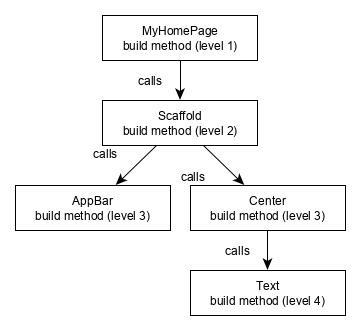
\includegraphics[width=0.7\textwidth]{Hinhve/Chuong5/widgettree.png}
    \caption{Sơ đồ cây widget}
    \label{fig:widgettree}
\end{figure}
Quá trình dựng UI thông qua \texttt{build()} trong Flutter có thể chia thành hai giai đoạn chính:

\textbf{1. Giai đoạn khởi tạo (Initial Build):}
\begin{itemize}
\item Khi một widget (chẳng hạn như \texttt{MyHomePage}) được chèn vào cây widget lần đầu tiên, Flutter sẽ gọi phương thức \texttt{build()} để xây dựng giao diện.
\item Trong ví dụ trên, phương thức \texttt{build()} trả về một widget \texttt{Scaffold}, sau đó tiếp tục gọi đệ quy để tạo các widget con: \texttt{AppBar}, \texttt{Center}, và cuối cùng là hai \texttt{Text} widget.
\item Quá trình này có tính chất đệ quy – mỗi widget cha tạo ra và xây dựng các widget con của nó trong cây.
\end{itemize}

\textbf{2. Giai đoạn cập nhật (Rebuild):}
\begin{itemize}
\item Với \texttt{StatelessWidget}, nếu các tham số truyền vào (như \texttt{title}) thay đổi, widget cũ sẽ bị loại bỏ và thay thế bằng một widget mới → khi đó \texttt{build()} được gọi lại để dựng lại cây giao diện tương ứng.
\item Với \texttt{StatefulWidget}, khi gọi phương thức \texttt{setState()}, Flutter đánh dấu widget cần được cập nhật. Khi đến khung hình tiếp theo (frame), Flutter sẽ gọi lại \texttt{build()} cho widget đó để cập nhật giao diện phù hợp với trạng thái mới.
\item Ngoài ra, nếu một \texttt{InheritedWidget} (là một widget chứa thông tin chia sẻ cho các widget con) mà widget đang phụ thuộc vào bị thay đổi, Flutter cũng sẽ tự động gọi lại \texttt{build()} của các widget con bị ảnh hưởng.
\end{itemize}

\textbf{Tính hiệu quả và ưu điểm:}

Việc sử dụng mô hình khai báo kết hợp với phương thức \texttt{build()} mang lại nhiều lợi ích:
\begin{itemize}
\item \textbf{Tăng khả năng đọc và bảo trì mã nguồn:} Cấu trúc widget dạng cây dễ hình dung và gắn liền trực tiếp với giao diện. Nhờ đó, lập trình viên có thể dễ dàng hình dung và điều chỉnh bố cục ứng dụng chỉ bằng cách đọc mã.
\item \textbf{Giảm thiểu lỗi cập nhật giao diện:} Thay vì phải tự mình cập nhật từng phần giao diện khi dữ liệu thay đổi (như trong lập trình mệnh lệnh), lập trình viên chỉ cần mô tả trạng thái mong muốn. Flutter sẽ tự động xử lý các thay đổi và dựng lại giao diện phù hợp, hạn chế tối đa lỗi logic hoặc thiếu sót khi cập nhật UI.
\item \textbf{Hỗ trợ công cụ Hot Reload mạnh mẽ trong Flutter:} Vì toàn bộ giao diện được xác định bởi phương thức \texttt{build()}, Flutter có thể tái tạo lại nhanh chóng khi mã thay đổi. Điều này giúp lập trình viên thử nghiệm và kiểm tra giao diện gần như ngay lập tức mà không cần khởi động lại ứng dụng.
\end{itemize}

\textbf{Hiệu suất và tối ưu hóa khi sử dụng \texttt{build()}:}

Để đảm bảo hiệu năng cao khi ứng dụng phát triển phức tạp hơn, Flutter triển khai nhiều cơ chế tối ưu liên quan đến cách \texttt{build()} được gọi và xử lý:
\begin{itemize}
\item \textbf{Cơ chế so sánh (reconciliation):} Khi phương thức \texttt{build()} được gọi, Flutter sẽ so sánh cây widget mới với cây cũ để phát hiện sự thay đổi. Chỉ những widget thực sự bị thay đổi mới được dựng lại hoặc cập nhật trên màn hình, nhờ đó tránh lãng phí tài nguyên không cần thiết. 
\item \textbf{Tránh đặt logic nặng trong \texttt{build()}:} Vì \texttt{build()} có thể được gọi lại thường xuyên, nên không nên thực hiện các tác vụ tốn tài nguyên như truy vấn cơ sở dữ liệu, xử lý phức tạp, hoặc gọi API trực tiếp trong hàm này. Những công việc như vậy nên được xử lý ở nơi khác (ví dụ như trong \texttt{initState()} hoặc khi người dùng tương tác), để tránh ảnh hưởng đến tốc độ phản hồi của giao diện.
\item \textbf{Tách widget hợp lý để giới hạn phạm vi rebuild:} Một cách tối ưu phổ biến là chia nhỏ các phần giao diện thành các widget con riêng biệt, nhất là những phần thường xuyên thay đổi. Điều này giúp giới hạn khu vực cần tái dựng khi trạng thái thay đổi, đồng thời tăng khả năng tái sử dụng và kiểm soát logic tốt hơn.
\end{itemize}

\section{Quản lí trạng thái trong Flutter}
\textbf{Quản lý trạng thái (state management)} là một trong những yếu tố cốt lõi và không thể thiếu trong vòng đời của một ứng dụng Flutter. Trạng thái là bất kỳ dữ liệu nào có thể thay đổi trong quá trình chạy ứng dụng và ảnh hưởng đến cách giao diện người dùng được hiển thị. Do Flutter áp dụng mô hình UI khai báo, mỗi khi trạng thái thay đổi, UI sẽ cần được xây dựng lại để phản ánh sự thay đổi đó. Do đó, cách quản lý trạng thái hiệu quả sẽ quyết định đến hiệu suất, khả năng mở rộng và độ ổn định của ứng dụng.

\textbf{Phân loại trạng thái:}

Trong Flutter, state có thể được chia thành hai nhóm chính:
\begin{itemize}
\item \textbf{Local state (trạng thái cục bộ): } Là trạng thái chỉ tồn tại trong phạm vi một widget duy nhất. Nó thường liên quan đến những thay đổi nhỏ trên UI như tab hiện tại đang chọn, checkbox được tích hay không, giá trị của một biến boolean,... Trạng thái này thường được quản lý bằng \texttt{StatefulWidget}.
\item \textbf{Application State (trạng thái toàn cục)}: Là loại trạng thái không cục bộ, được chia sẻ giữa nhiều widget hoặc tồn tại xuyên suốt vòng đời của phiên làm việc của người dùng. Ví dụ như thông tin đăng nhập, danh sách sản phẩm trong giỏ hàng, tin nhắn trò chuyện,... Trạng thái này thường yêu cầu các giải pháp quản lý state phức tạp hơn như Provider, Riverpod, Bloc, Redux,...
\end{itemize}

Cách một widget xử lý và phản ứng với trạng thái được quyết định bởi việc nó là Stateless hay Stateful.
\begin{figure}[H]
    \centering
    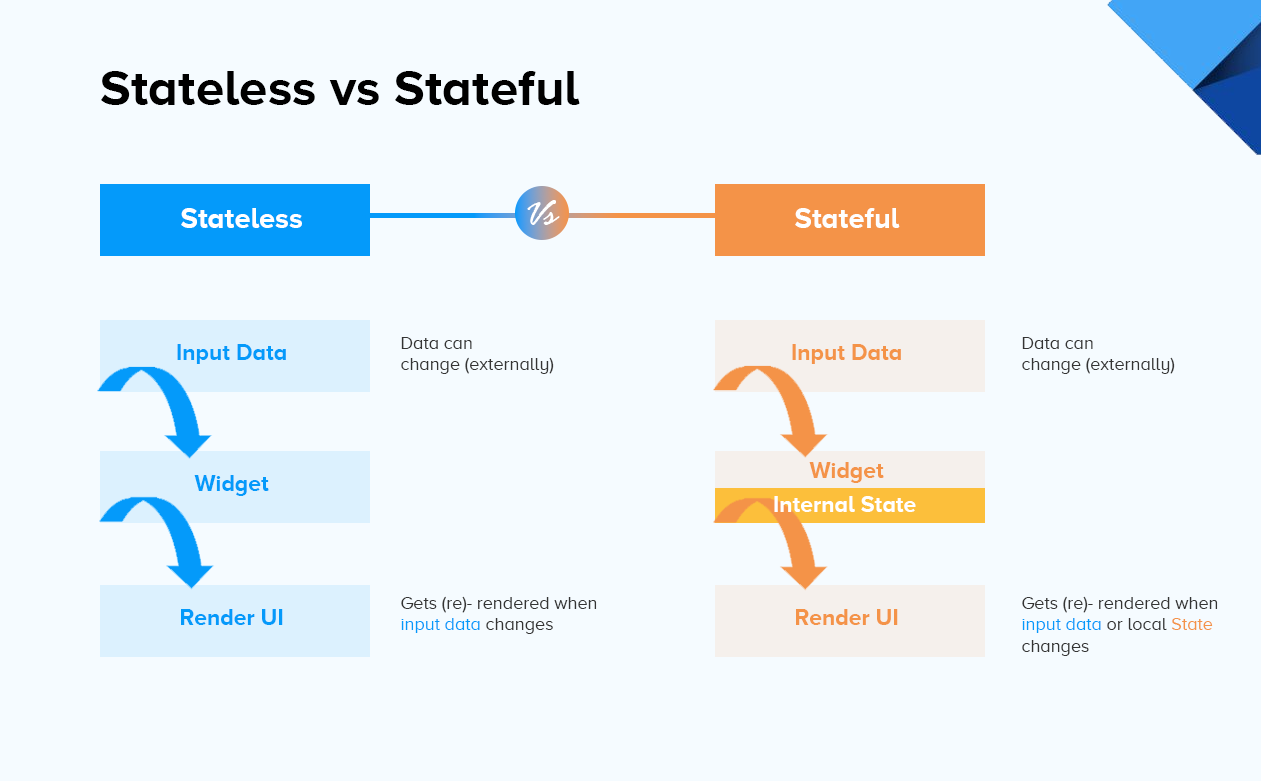
\includegraphics[width=0.7\textwidth]{Hinhve/Chuong5/stlessvastful.png}
    \caption{Trạng thái của Widget}
    \label{fig:stlessvastful}
\end{figure}

\subsection{Stateless Widget}
\textbf{Stateless widget} là một widget không quản lý trạng thái của chính nó. Khi được khởi tạo, nó nhận các tham số đầu vào thông qua Constructor và chỉ hiển thị UI dựa trên những giá trị đó. Nếu muốn thay đổi thì toàn bộ widget phải được tái tạo từ đầu với tham số mới. Bản thân \textbf{Stateless widget} cũng không có hàm createState mà thay vào đó là hàm build(BuildContext)

\textbf{Vòng đời của Stateless Widget} bao gồm hai giai đoạn cơ bản:

\begin{enumerate}
\item \textbf{Constructor được gọi:} Khi widget được thêm vào cây widget, Flutter khởi tạo một thể hiện mới bằng constructor, nhận các tham số từ widget cha.
\item \textbf{Phương thức \texttt{build()} được gọi:} Ngay sau khi khởi tạo, Flutter gọi phương thức \texttt{build(BuildContext context)} để dựng cây widget con, mô tả cách giao diện của widget này sẽ hiển thị.
\end{enumerate}
\begin{figure}[H]
    \centering
    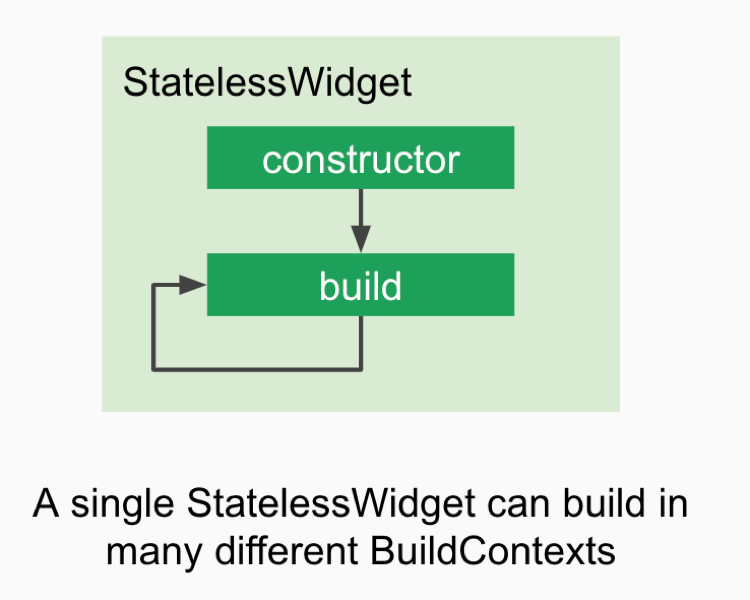
\includegraphics[width=0.8\textwidth]{Hinhve/Chuong5/statelesswidgetimg.png}
    \caption{Vòng đời của StatelessWidget}
    \label{fig:statelesswidgetimg}
\end{figure}
Như sơ đồ minh họa, StatelessWidget được khởi tạo thông qua constructor và chỉ thực hiện một hành vi duy nhất là gọi hàm \texttt{build()} để trả về cấu trúc giao diện. Sau đó, nó không tự thay đổi hoặc cập nhật bất kỳ phần tử nào.

\textbf{Ví dụ về Stateless Widget:}
\begin{lstlisting}
Text(
    'Hello, Flutter!', 
    style: TextStyle(
        fontSize: 20, 
        color: Colors.blue
    )
)
\end{lstlisting}


Ở ví dụ trên, \texttt{Text} là một widget bất biến, nó chỉ hiển thị văn bản được truyền vào, nếu cần thay đổi nội dung thì cần phải tạo lại một widget \texttt{Text} mới với nội dung khác.

\subsection{Stateful widget}
Trái ngược với Stateless Widget, một \textbf{Stateful Widget} là loại widget có khả năng quản lý trạng thái nội tại (internal state) và tự động cập nhật giao diện khi trạng thái thay đổi. Điều này khiến StatefulWidget rất hữu ích trong các tình huống tương tác động hoặc khi dữ liệu hiển thị cần thay đổi linh hoạt theo thời gian.

\textbf{Stateful Widget} không chỉ có phương thức \texttt{build()} mà còn có đối tượng State được liên kết xác định một số phương thức để hỗ trợ vòng đời của Widget. Chính đối tượng \texttt{State} này mới là nơi lưu trữ và quản lý trạng thái động của widget. Việc thay đổi trạng thái được thực hiện thông qua phương thức \texttt{setState()}, giúp Flutter biết rằng giao diện cần được cập nhật lại.
\texttt{StatefulWidget} cho phép giao diện thay đổi dựa trên hành động của người dùng, dữ liệu động hoặc sự kiện bất đồng bộ.

\textbf{Cấu trúc tổng quát của Stateful widget:}

\begin{lstlisting}
class MyWidget extends StatefulWidget {
    @override
    State<MyWidget> createState() => _MyWidgetState();
}

class _MyWidgetState extends State<MyWidget> {
    @override
    Widget build(BuildContext context) {
        return Container(); 
    }
}
\end{lstlisting}

Lớp \textbf{\texttt{MyWidget}} kế thừa từ \texttt{StatefulWidget} đại diện cho phần cấu hình không đổi của widget. Lớp \textbf{\texttt{\_MyWidgetState}} kế thừa từ \texttt{State<MyWidget>} lưu trữ dữ liệu thay đổi và triển khai giao diện.

\textbf{Vòng đời của Stateful widget:}

\textbf{Stateful Widget} có một loạt các phương thức vòng đời trong lớp State, cho phép can thiệp vào từng giai đoạn hoạt động của widget.
\begin{figure}[H]
    \centering
    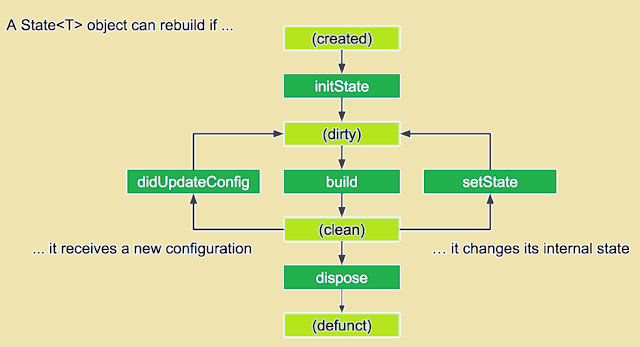
\includegraphics[width=0.8\textwidth]{Hinhve/Chuong5/statefulwidgetimg.png}
    \caption{Vòng đời của Stateful Widget}
    \label{fig:statefulwidgetimg}
\end{figure}

\begin{itemize}
\item \textbf{\texttt{createState():}} Khi một widget được thêm vào cây widget, Flutter sẽ gọi \texttt{createState()} để tạo một đối tượng trạng thái tương ứng. Đối tượng \texttt{State} này sau đó sẽ được giữ cố định trong suốt vòng đời của widget (trừ khi widget bị loại bỏ vĩnh viễn).

\item \textbf{\texttt{initState():}} Là phương thức đầu tiên được gọi trong lớp \texttt{State}, nó chỉ được gọi duy nhất một lần, ngay sau khi \texttt{createState()} hoàn tất và trước khi widget được dựng giao diện. Đây là nơi để khởi tạo các dữ liệu cần thiết, đăng ký lắng nghe sự kiện (listener), thiết lập controller, hoặc bất kỳ công việc nào cần thực hiện một lần duy nhất khi widget được đưa vào cây.

\item \textbf{\texttt{didChangeDependencies()}:}
Sau phương thức \texttt{initState()}, Flutter gọi \texttt{didChangeDependencies()} nếu widget phụ thuộc vào một hoặc nhiều đối tượng kế thừa (\texttt{InheritedWidget}). Phương thức này cũng có thể được gọi lại nếu một \texttt{InheritedWidget} mà widget đang phụ thuộc bị thay đổi. Đây là nơi phù hợp để truy xuất các giá trị phụ thuộc từ context.

\item \textbf{\texttt{build()}:}
Là phương thức cốt lõi của bất kỳ widget nào. Nó được gọi mỗi khi Flutter cần dựng lại giao diện dựa trên trạng thái hiện tại. Mỗi lần \texttt{setState()} được gọi hoặc cấu hình widget thay đổi từ widget cha, Flutter sẽ tự động gọi lại \texttt{build()}. \texttt{BuildContext} được truyền vào để cho biết vị trí của widget trong cây widget, đồng thời cho phép truy xuất các widget tổ tiên như \texttt{Theme}, \texttt{MediaQuery}, hoặc \texttt{Provider}.

\item \textbf{\texttt{setState()}:}
Là cơ chế mà thông qua đó Flutter biết được rằng trạng thái nội tại của widget đã thay đổi. Khi gọi \texttt{setState(callback)}, Flutter sẽ đánh dấu widget là “dirty” và lập lịch gọi lại \texttt{build()} trong khung hình tiếp theo. 

\item \textbf{\texttt{didUpdateWidget()}:}
Được gọi khi widget cha rebuild và truyền một phiên bản mới của widget con có cùng \texttt{runtimeType} nhưng khác cấu hình. Flutter sẽ tái sử dụng đối tượng \texttt{State} hiện tại thay vì tạo mới, và phương thức này sẽ cung cấp quyền truy cập vào phiên bản widget cũ để so sánh và xử lý sự thay đổi.

\item \textbf{\texttt{deactivate()}:}
Được gọi khi widget tạm thời bị loại khỏi cây widget, điều này có thể xảy ra khi điều hướng sang màn hình khác. Widget vẫn có thể được tái chèn lại nếu quay trở về màn hình trước trong cùng khung hình. 

\item \textbf{\texttt{dispose()}:}
Là phương thức cuối cùng được gọi trong vòng đời. Flutter gọi \texttt{dispose()} khi widget bị loại bỏ vĩnh viễn khỏi cây widget. Đây là nơi cần giải phóng tài nguyên như controller, stream, animation, hoặc subscription để tránh rò rỉ bộ nhớ. 
\end{itemize}

Xét ví dụ \textbf{CounterApp:} Một ứng dụng đơn giản với giao diện gồm một nút bấm ở góc dưới bên phải màn hình. Mỗi lần người dùng nhấn nút “+”, số đếm hiển thị ở giữa màn hình sẽ tăng lên một đơn vị. 
\begin{figure}[H]
    \centering
    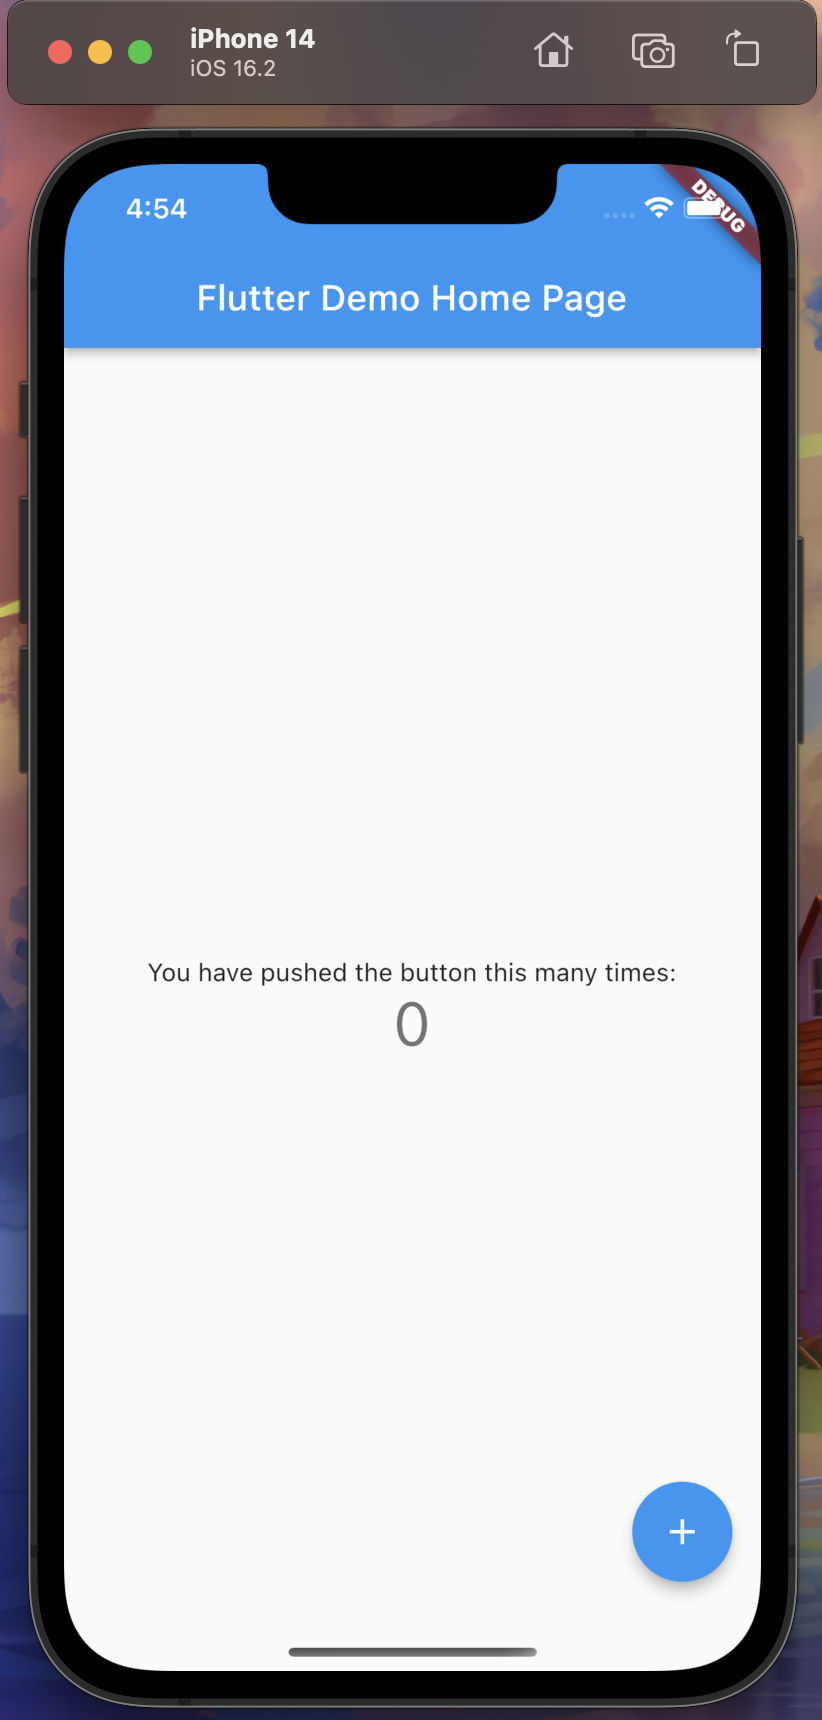
\includegraphics[width=0.5\textwidth]{Hinhve/Chuong5/counterapp.png}
    \caption{Counter App Demo}
    \label{fig:counterapp}
\end{figure}

Mã nguồn được tổ chức thành hai lớp:
\begin{itemize}
\item \textbf{\texttt{ MyHomePage}} kế thừa từ \texttt{StatefulWidget}, đóng vai trò là lớp cấu hình.
\item \textbf{\texttt{ \_MyHomePageState}} kế thừa từ \texttt{State<MyHomePage>}, lưu trữ trạng thái động và định nghĩa giao diện.
\end{itemize}

\begin{lstlisting}
class MyHomePage extends StatefulWidget {
  MyHomePage({Key? key, required this.title}) : super(key: key);
  final String title;

  @override
  _MyHomePageState createState() => _MyHomePageState();
}

class _MyHomePageState extends State<MyHomePage> {
  int _counter = 0;

  void _incrementCounter() {
    setState(() {
      _counter++;
    });
  }

  @override
  Widget build(BuildContext context) {
    return Scaffold(
      appBar: AppBar(title: Text(widget.title)),
      body: Center(
        child: Column(
          mainAxisAlignment: MainAxisAlignment.center,
          children: <Widget>[
            Text('You have pushed the button this many times:'),
            Text('$_counter',
                style: Theme.of(context).textTheme.headlineMedium),
          ],
        ),
      ),
      floatingActionButton: FloatingActionButton(
        onPressed: _incrementCounter,
        tooltip: 'Increment',
        child: const Icon(Icons.add),
      ),
    );
  }
}
\end{lstlisting}

\textbf{Phân tích hoạt động theo vòng đời:}

\begin{itemize}
\item \textbf{Giai đoạn khởi tạo: } Khi ứng dụng chạy, Flutter gọi  \texttt{createState()} từ lớp \textbf{\texttt{MyHomePage}}, trả về một thể hiện của \textbf{\texttt{\_MyHomePageState}}. Sau đó Flutter gọi \texttt{initState()} trong \texttt{State} để khởi tạo trạng thái ban đầu của biến \texttt{\_counter} là 0.
\item \textbf{Giai đoạn dựng UI: } Ngay sau \texttt{initState()}, Flutter gọi \texttt{build()} để tạo giao diện lần đầu. Kết quả là một giao diện hiển thị số lần nhấn nút.
\item \textbf{Tương tác người dùng: } Khi người dùng nhấn vào nút “+”, hàm \texttt{\_incrementCounter()} được gọi, bên trong đó có gọi \texttt{setState()}. Lệnh \texttt{setState()} báo cho Flutter biết rằng trạng thái \texttt{\_counter} đã thay đổi → giao diện cần được cập nhật. Flutter đánh dấu widget là “dirty” và trong khung hình tiếp theo, nó sẽ gọi lại phương thức \texttt{build()} để hiển thị giá trị mới.
\end{itemize}

Ta có thể thấy rõ sự liên kết giữa các giai đoạn trong vòng đời và hoạt động thực tế của widget: \texttt{initState()} và \texttt{build()} xuất hiện khi khởi tạo widget, \texttt{setState()} là cầu nối giữa thay đổi dữ liệu và cập nhật UI, \texttt{build()} được gọi lại mỗi khi trạng thái thay đổi nhưng không đồng nghĩa với việc toàn bộ giao diện bị dựng lại.

\subsection{Các giải pháp quản lý trạng thái ứng dụng}
Qua ví dụ \texttt{CounterApp} đã trình bày, có thể thấy rõ rằng phương thức \texttt{setState()} là một giải pháp đơn giản, hiệu quả cho việc quản lý trạng thái cục bộ (\textit{Local state}) trong Flutter. Khi người dùng tương tác (ví dụ như nhấn nút “+”), hàm \texttt{\_incrementCounter()} được gọi, và bên trong nó thực thi \texttt{setState()} để cập nhật biến \texttt{\_counter}. Nhờ đó, Flutter đánh dấu lại widget tương ứng là “dirty” và tự động gọi lại phương thức \texttt{build()} để làm mới phần giao diện.

Tuy nhiên, khi phát triển các ứng dụng phức tạp hơn, việc quản lý trạng thái trở nên thách thức. Cụ thể, nếu một trạng thái cần được chia sẻ giữa nhiều widget nằm rải rác trong cây giao diện, việc sử dụng thuần túy \texttt{setState()} không còn đủ hiệu quả. Trạng thái có thể bị truyền qua nhiều tầng widget không liên quan (hiện tượng gọi là \textit{prop drilling}), khiến cho mã nguồn trở nên khó đọc, khó bảo trì và dễ phát sinh lỗi không mong muốn.

Một cách tiếp cận ban đầu là đặt trạng thái trong một widget cha đủ lớn, rồi truyền dữ liệu cho các widget con cần sử dụng thông qua constructor hoặc phương thức. Tuy nhiên, cách này nảy sinh một số vấn đề. Thứ nhất, các widget không sử dụng trạng thái cũng có thể bị \texttt{rebuild} do ảnh hưởng từ widget cha. Thứ hai, mã nguồn của widget cha trở nên cồng kềnh và khó tách biệt giữa giao diện và logic xử lý. Cuối cùng, khi ứng dụng có các logic nghiệp vụ cần kiểm tra, việc kiểm thử trở nên khó khăn nếu mọi thứ được ràng buộc trực tiếp vào widget UI.

Để giải quyết các bất cập trên, Flutter cung cấp nhiều cơ chế và thư viện hỗ trợ quản lý \textit{Application state} – trạng thái dùng chung trên toàn bộ hoặc nhiều phần của giao diện. Đây là các giải pháp giúp tách biệt dữ liệu và UI, đồng thời tối ưu hiệu suất bằng cách giới hạn vùng ảnh hưởng khi trạng thái thay đổi.

Một trong những lớp nền tảng được sử dụng là \textbf{\texttt{InheritedWidget}}. Đây là một widget đặc biệt cho phép truyền dữ liệu từ trên xuống dưới qua cây widget, và các widget con có thể truy cập dữ liệu đó bằng phương thức \texttt{of(context)}. Tuy nhiên, việc sử dụng \textbf{\texttt{InheritedWidget}} trực tiếp thường không thân thiện với lập trình viên mới, do đó nhiều thư viện đã được xây dựng trên nền tảng này để đơn giản hóa việc quản lý trạng thái.

Các thư viện phổ biến hiện nay:

\begin{itemize}
    \item \textbf{Provider}: Một thư viện được cộng đồng sử dụng rộng rãi, cung cấp một cách tiếp cận đơn giản nhưng mạnh mẽ để chia sẻ và giám sát trạng thái.
    \item \textbf{BLoC (Business Logic Component)}: Áp dụng mô hình lập trình phản ứng (reactive programming), giúp tách biệt hoàn toàn logic xử lý và giao diện bằng cách sử dụng luồng dữ liệu (Streams).
    \item \textbf{flutter\_bloc}: Một gói mở rộng dựa trên BLoC, cung cấp các widget sẵn có giúp dễ dàng tích hợp và sử dụng.
    \item \textbf{Redux}: Mô hình quản lý trạng thái một chiều, lấy cảm hứng từ React Redux, phù hợp với các ứng dụng lớn và có luồng dữ liệu phức tạp.
    \item \textbf{MobX}: Một thư viện dựa trên nguyên lý lập trình phản ứng tự động (\textit{observable}), giúp theo dõi và tự động cập nhật giao diện khi dữ liệu thay đổi.
\end{itemize}

\begin{figure}[H]
    \centering
    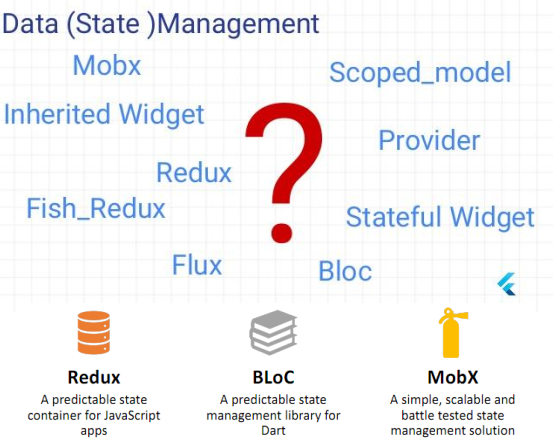
\includegraphics[width=0.8\textwidth]{Hinhve/Chuong5/statemanagement.png}
    \caption{Các giải pháp quản lý trạng thái ứng dụng}
    \label{fig:statemanagement}
\end{figure}

\section{RenderObject và RenderTree}
Trong Flutter, việc xây dựng giao diện người dùng (UI) không chỉ đơn thuần là tạo ra các widget. Thay vào đó, Flutter tổ chức hệ thống UI thành ba tầng logic: \textbf{Widget Tree}, \textbf{Element Tree} và \textbf{Render Tree}. Mỗi tầng đảm nhận một vai trò cụ thể, giúp tối ưu hóa hiệu suất, quản lý vòng đời giao diện và đảm bảo tính linh hoạt khi phát triển ứng dụng.

\begin{figure}[H]
    \centering
    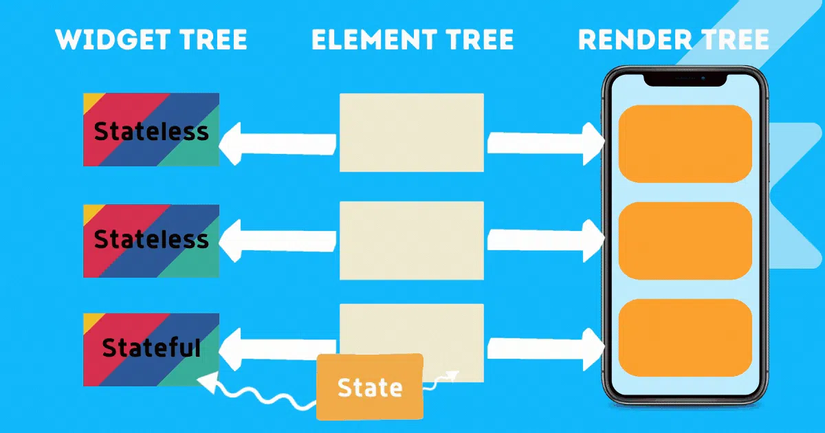
\includegraphics[width=0.8\textwidth]{Hinhve/Chuong5/treeflutter.png}
    \caption{Các tầng Logic trong hệ thống UI của Flutter}
    \label{fig:treeflutter}
\end{figure}

\subsection{Khái niệm}

\textbf{Widget Tree} là tập hợp các widget, được xem như các khối xây dựng cơ bản của giao diện trong Flutter. Widgets là các đối tượng bất biến (immutable), đóng vai trò mô tả cấu hình của UI, chẳng hạn như bố cục, màu sắc hoặc nội dung. Tuy nhiên, widgets không trực tiếp thực hiện việc render mà chỉ cung cấp thông tin cần thiết cho các tầng khác. Khi các widget được lồng ghép, chúng tạo thành một cấu trúc cây gọi là Widget Tree.

\textbf{Element Tree} được tạo ra từ Widget Tree và đóng vai trò trung gian trong việc quản lý vòng đời của các widget. Mỗi element trong Element Tree tương ứng với một widget cụ thể và tham chiếu đến widget đó để truy cập cấu hình. Elements chịu trách nhiệm so sánh các widget mới với các widget hiện có, từ đó quyết định cách cập nhật giao diện mà không cần tạo lại toàn bộ các đối tượng render. Ngoài ra, Elements còn quản lý trạng thái (state) của các widget, đảm bảo rằng các thay đổi trạng thái được phản ánh chính xác trên UI.

\textbf{Render Tree} là tầng cuối cùng, nơi diễn ra quá trình render thực tế. Nó bao gồm các \textbf{RenderObject}, là các đối tượng chịu trách nhiệm thực hiện layout (bố trí), painting (vẽ) và xử lý tương tác người dùng trên màn hình. RenderObjects xác định các thuộc tính như kích thước, vị trí, hình học và nội dung của từng thành phần UI. Mỗi Element trong Element Tree trỏ đến một
RenderObject trong Render Tree, đóng vai trò cầu nối giữa cấu hình và hiển thị
thực tế. Chúng cũng hỗ trợ \textit{hit testing}, giúp xác định các khu vực trên màn hình có thể phản hồi các cử chỉ như chạm, vuốt hoặc kéo. 

\textbf{RenderObject} là thành phần cốt lõi của Render Tree. Mỗi RenderObject đại diện cho một phần của giao diện và biết cách tự bố trí (layout) bản thân cũng như các con của nó, đồng thời thực hiện việc vẽ (paint) lên màn hình. Ví dụ, một RenderObject như \texttt{RenderOpacity} có thể bọc một RenderObject khác và áp dụng hiệu ứng độ mờ trong quá trình vẽ.

Do chứa logic render phức tạp, RenderObjects là các đối tượng nặng (heavy), đòi hỏi nhiều tài nguyên tính toán. Vì vậy, Flutter tối ưu hóa bằng cách tái sử dụng RenderObjects hiện có thay vì tạo mới mỗi khi UI cần cập nhật. Các phương thức như \texttt{markNeedsPaint()} hoặc \texttt{markNeedsLayout()} được sử dụng để báo hiệu rằng một RenderObject cần được vẽ lại hoặc bố trí lại.

Render Tree hoạt động trong một hệ tọa độ độc lập với thiết bị (device-independent), sử dụng các pixel logic thay vì pixel vật lý. Điều này cho phép Flutter hiển thị giao diện nhất quán trên các thiết bị có độ phân giải và kích thước màn hình khác nhau.

\subsection{Mối quan hệ giữa các Tree}

\begin{figure}[H]
    \centering
    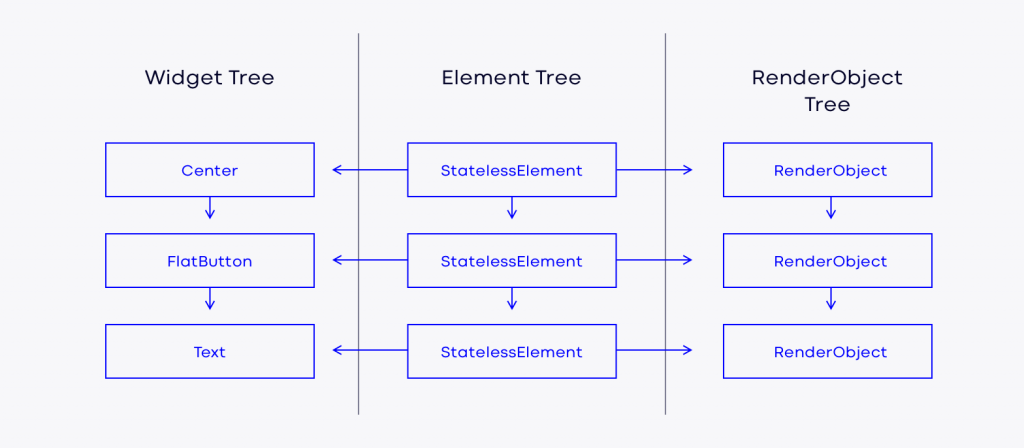
\includegraphics[width=0.9\textwidth]{Hinhve/Chuong5/3trees.png}
    \caption{Mối quan hệ giữa các cây}
    \label{fig:3trees}
\end{figure}

Ba cây phối hợp chặt chẽ để xây dựng và cập nhật giao diện một cách hiệu quả:
\begin{itemize}
    \item \textbf{Widget Tree}: Mô tả trạng thái mong muốn của UI thông qua các widget.
    \item \textbf{Element Tree}: Quản lý vòng đời và trạng thái, so sánh các widget mới với các widget hiện có để xác định các thay đổi cần thiết.
    \item \textbf{Render Tree}: Thực hiện render dựa trên cấu hình từ Element Tree, sử dụng các RenderObject để vẽ giao diện.
\end{itemize}

Sự phân tách này mang lại hiệu quả cao. Khi một widget trong Widget Tree thay đổi, element tương ứng trong Element Tree sẽ kiểm tra xem widget mới có cùng loại (\texttt{runtimeType}) với widget hiện có hay không. Nếu có, Flutter chỉ cập nhật cấu hình của RenderObject hiện tại thay vì tạo mới, giúp giảm thiểu chi phí tính toán. Nếu loại widget thay đổi, element sẽ phá hủy RenderObject cũ và tạo một RenderObject mới. 

Ví dụ, nếu một widget \texttt{Text} thay đổi nội dung từ ``Hello'' thành ``World'' nhưng vẫn giữ nguyên loại, element sẽ chỉ cập nhật thuộc tính văn bản của RenderObject tương ứng, thay vì tạo lại toàn bộ.

Khi người dùng tương tác với ứng dụng, ví dụ như khi nhấn vào một nút, sự tương tác này được xử lý bởi các gesture recognizers trong RenderObject. Các gesture recognizers này gọi các hàm callback được cung cấp bởi các widget, có thể cập nhật trạng thái của một widget trạng thái (stateful widget). Khi trạng thái thay đổi, widget được xây dựng lại, tạo ra một Widget Tree mới. Element Tree sau đó so sánh Widget Tree mới với Element Tree hiện tại để xác định những phần cần cập nhật, và cuối cùng, Render Tree được cập nhật để phản ánh các thay đổi trên màn hình.

Quá trình này được gọi là \textit{reconciliation}, đảm bảo rằng chỉ các phần cần thiết của giao diện được cập nhật, giảm thiểu chi phí tính toán và cải thiện hiệu suất.

\textbf{VÌ SAO CẦN ĐẾN BA CÂY?}

Flutter áp dụng mô hình ba cây vì các lý do sau:
\begin{itemize}
    \item \textbf{Hiệu suất}: Widgets nhẹ và có thể được tạo lại thường xuyên mà không tốn kém, trong khi RenderObjects nặng hơn và được tái sử dụng để tránh tạo lại không cần thiết.
    \item \textbf{Rõ ràng}: Mỗi cây có trách nhiệm riêng biệt, giúp mã nguồn dễ hiểu và dễ bảo trì. 
    \item \textbf{An toàn kiểu dữ liệu}: Sự phân tách ngăn chặn việc trộn lẫn logic giữa cấu hình và render, đảm bảo rằng các loại dữ liệu đúng được sử dụng trong từng ngữ cảnh.
\end{itemize}

\textbf{Ví dụ minh họa về sử dụng ba cây trong Flutter:}

Xét một ứng dụng Flutter đơn giản hiển thị văn bản ``Hello'' và một nút ``Change Content''. Khi người dùng nhấn nút, văn bản chuyển thành ``Welcome''.

\begin{itemize}
    \item \textbf{Widget Tree}: Bao gồm các widget như \texttt{Scaffold}, \texttt{Center}, \texttt{Column} với \texttt{Text} (văn bản) và \texttt{ElevatedButton} (nút ``Change Content'').
    \item \textbf{Element Tree}: Mỗi widget có element tương ứng. Widget chính là \texttt{StatefulWidget} quản lý nội dung văn bản.
    \item \textbf{Render Tree}: \texttt{RenderParagraph} cho \texttt{Text} và \texttt{RenderDecoratedBox} cho nút.
\end{itemize}

Khi người dùng nhấn nút ``Change Content'', trạng thái văn bản được cập nhật từ ``Hello'' sang ``Welcome''. Widget Tree được xây dựng lại với \texttt{Text} có nội dung mới. Element Tree so sánh và cập nhật element cho \texttt{Text}. Render Tree cập nhật \texttt{RenderParagraph} để vẽ văn bản mới.Chỉ phần \texttt{Text} được vẽ lại, các phần khác không bị ảnh hưởng. Quy trình này đảm bảo rằng chỉ các phần cần thiết được cập nhật, tối ưu hóa hiệu suất
\end{document} 